% ═══════════════════════════════════════════════════════════════════════════════
% Pearls AQI Predictor - Technical Documentation
% Author: Zain ul Abdeen
% Date: August 2026
% ═══════════════════════════════════════════════════════════════════════════════

\documentclass[12pt, a4paper, oneside]{report}

% ── Packages ──────────────────────────────────────────────────────────────────
\usepackage[utf8]{inputenc}
\usepackage[T1]{fontenc}
\usepackage{lmodern}
\usepackage[margin=2.5cm, headheight=15pt]{geometry}
\usepackage{graphicx}
\usepackage{xcolor}
\usepackage{hyperref}
\usepackage{booktabs}
\usepackage{longtable}
\usepackage{tabularx}
\usepackage{float}
\usepackage{amsmath}
\usepackage{amssymb}
\usepackage{listings}
\usepackage{fancyhdr}
\usepackage{titlesec}
\usepackage{tocloft}
\usepackage{enumitem}
\usepackage{multirow}
\usepackage{caption}
\usepackage{subcaption}
\usepackage{tikz}
\usetikzlibrary{positioning, arrows.meta}
\usepackage{pgfplots}
\pgfplotsset{compat=1.18}
\usepackage{tcolorbox}
\tcbuselibrary{listingsutf8, skins, breakable}
\raggedbottom

% ── Graphics Path ─────────────────────────────────────────────────────────────
\graphicspath{{../eda/plots/}}

% ── Colors ────────────────────────────────────────────────────────────────────
\definecolor{primaryblue}{RGB}{41, 128, 185}
\definecolor{darkblue}{RGB}{23, 37, 84}
\definecolor{accentgreen}{RGB}{39, 174, 96}
\definecolor{codebg}{RGB}{245, 245, 250}
\definecolor{codeframe}{RGB}{200, 200, 220}
\definecolor{warnorange}{RGB}{230, 126, 34}
\definecolor{dangerred}{RGB}{231, 76, 60}

% ── Hyperref Setup ────────────────────────────────────────────────────────────
\hypersetup{
    colorlinks=true,
    linkcolor=primaryblue,
    urlcolor=primaryblue,
    citecolor=accentgreen,
    pdftitle={Pearls AQI Predictor - Technical Documentation},
    pdfauthor={Zain ul Abdeen},
    pdfsubject={Air Quality Index Forecasting System},
}

% ── Code Listing Style ────────────────────────────────────────────────────────
\lstdefinestyle{pythonstyle}{
    language=Python,
    basicstyle=\ttfamily\small,
    backgroundcolor=\color{codebg},
    frame=single,
    rulecolor=\color{codeframe},
    keywordstyle=\color{primaryblue}\bfseries,
    commentstyle=\color{gray},
    stringstyle=\color{accentgreen},
    showstringspaces=false,
    breaklines=true,
    numbers=left,
    numberstyle=\tiny\color{gray},
    numbersep=8pt,
    tabsize=4,
}
\lstset{style=pythonstyle}

% ── Header/Footer ─────────────────────────────────────────────────────────────
\pagestyle{fancy}
\fancyhf{}
\fancyhead[L]{\small\textcolor{gray}{Pearls AQI Predictor}}
\fancyhead[R]{\small\textcolor{gray}{Technical Documentation}}
\fancyfoot[C]{\thepage}
\renewcommand{\headrulewidth}{0.4pt}

% ── Chapter/Section Formatting ────────────────────────────────────────────────
\titleformat{\chapter}[display]
  {\normalfont\huge\bfseries\color{darkblue}}
  {\chaptertitlename\ \thechapter}{20pt}{\Huge}
\titleformat{\section}
  {\normalfont\Large\bfseries\color{primaryblue}}
  {\thesection}{1em}{}
\titleformat{\subsection}
  {\normalfont\large\bfseries\color{darkblue}}
  {\thesubsection}{1em}{}

% ── Custom Box Environments ───────────────────────────────────────────────────
\newtcolorbox{infobox}[1][]{
    colback=primaryblue!5,
    colframe=primaryblue!75,
    fonttitle=\bfseries,
    title=#1,
    breakable,
}

\newtcolorbox{warnbox}[1][]{
    colback=warnorange!5,
    colframe=warnorange!75,
    fonttitle=\bfseries,
    title=#1,
    breakable,
}

% ═══════════════════════════════════════════════════════════════════════════════
\begin{document}

% ── Title Page ────────────────────────────────────────────────────────────────
\begin{titlepage}
\begin{center}

\vspace*{-1cm}

% Top decorative band
\noindent\begin{tikzpicture}[remember picture, overlay]
    \fill[darkblue] (current page.north west) rectangle ([yshift=-4cm]current page.north east);
    \fill[primaryblue] ([yshift=-4cm]current page.north west) rectangle ([yshift=-4.15cm]current page.north east);
    \fill[accentgreen] ([yshift=-4.15cm]current page.north west) rectangle ([yshift=-4.25cm]current page.north east);
\end{tikzpicture}

\vspace{2cm}

{\color{white}\Huge\bfseries Pearls AQI Predictor}

\vspace{0.3cm}

{\color{white}\Large End-to-End Air Quality Forecasting System}

\vspace{3.5cm}

% Central decorative element
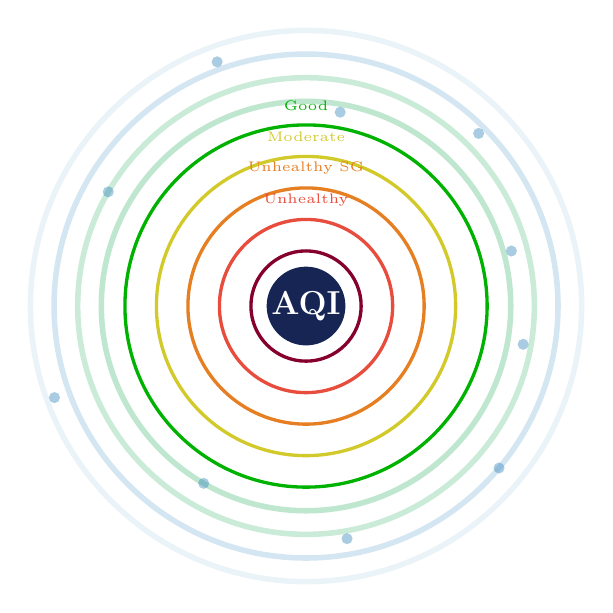
\begin{tikzpicture}
    % Outer glow rings
    \foreach \r/\c/\o in {3.5/primaryblue/10, 3.2/primaryblue/20, 2.9/accentgreen/25, 2.6/accentgreen/30} {
        \draw[\c, opacity=\o/100, line width=2pt] (0,0) circle (\r cm);
    }
    % Main rings representing AQI levels
    \draw[green!70!black, very thick] (0,0) circle (2.3cm);
    \draw[yellow!80!black, very thick] (0,0) circle (1.9cm);
    \draw[warnorange, very thick] (0,0) circle (1.5cm);
    \draw[dangerred, very thick] (0,0) circle (1.1cm);
    \draw[purple!70!black, very thick] (0,0) circle (0.7cm);
    % Center
    \fill[darkblue] (0,0) circle (0.5cm);
    \node[font=\large\bfseries, text=white] at (0,0) {AQI};
    % Labels around
    \node[font=\tiny, text=green!70!black] at (0, 2.55) {Good};
    \node[font=\tiny, text=yellow!80!black] at (0, 2.15) {Moderate};
    \node[font=\tiny, text=warnorange] at (0, 1.75) {Unhealthy SG};
    \node[font=\tiny, text=dangerred] at (0, 1.35) {Unhealthy};
    % Data points scattered
    \foreach \a/\r in {15/2.7, 45/3.1, 80/2.5, 110/3.3, 150/2.9, 200/3.4, 240/2.6, 280/3.0, 320/3.2, 350/2.8} {
        \fill[primaryblue, opacity=0.4] (\a:\r cm) circle (2pt);
    }
\end{tikzpicture}

\vspace{1.5cm}

% Project details box
\begin{tcolorbox}[
    colback=primaryblue!3,
    colframe=primaryblue!50,
    width=12cm,
    arc=4mm,
    boxrule=0.5pt,
]
\centering
\begin{tabular}{rl}
    \textcolor{primaryblue}{\textbf{Target:}} & Sargodha, Pakistan (32.08\textdegree N, 72.67\textdegree E) \\[3pt]
    \textcolor{primaryblue}{\textbf{Horizon:}} & 72-Hour (3-Day) AQI Forecast \\[3pt]
    \textcolor{primaryblue}{\textbf{Models:}} & 9 ML Models (Linear $\rightarrow$ Deep Learning) \\[3pt]
    \textcolor{primaryblue}{\textbf{Pipeline:}} & Hourly Ingestion + Daily Training (GitHub Actions) \\[3pt]
    \textcolor{primaryblue}{\textbf{Stack:}} & Python, Flask, Next.js, PyTorch, ClearML \\[3pt]
    \textcolor{primaryblue}{\textbf{Deployment:}} & Render (API) + Vercel (Frontend) \\[3pt]
    \textcolor{primaryblue}{\textbf{Explainability:}} & SHAP + LIME + Temporal Grad-CAM \\
\end{tabular}
\end{tcolorbox}

\vfill

% Bottom section

\begin{tikzpicture}[remember picture, overlay]
    \fill[darkblue] (current page.south west) rectangle ([yshift=2.5cm]current page.south east);
    \fill[primaryblue] ([yshift=2.5cm]current page.south west) rectangle ([yshift=2.65cm]current page.south east);
    \fill[accentgreen] ([yshift=2.65cm]current page.south west) rectangle ([yshift=2.75cm]current page.south east);
\end{tikzpicture}

\vspace{0.5cm}

{\color{white}\large\textbf{Zain ul Abdeen}}

\vspace{0.15cm}

{\color{white}\normalsize Pearls Engineering Program | August 2026 | v2.0.0}

\vspace{1cm}

\end{center}
\end{titlepage}

% ── Table of Contents ─────────────────────────────────────────────────────────
\tableofcontents
\newpage

% ── List of Figures & Tables ──────────────────────────────────────────────────
\listoffigures
\listoftables
\newpage

% ═══════════════════════════════════════════════════════════════════════════════
\chapter{Introduction}
% ═══════════════════════════════════════════════════════════════════════════════

\section{Project Overview}

The Pearls AQI Predictor is a production-ready, end-to-end machine learning system that forecasts Air Quality Index (AQI) \textbf{72 hours (3 days)} into the future for Sargodha, Pakistan. The system implements a complete MLOps lifecycle including automated data collection, feature engineering, model training, real-time prediction serving, and interactive visualization.

\begin{infobox}[Key Objectives]
\begin{itemize}[noitemsep]
    \item Predict AQI for the next 3 days using 9 distinct model architectures
    \item Automate data collection from AQICN and OpenWeatherMap APIs
    \item Train, version, and serve all 9 models through a dynamic model zoo
    \item Provide model explainability via SHAP and LIME
    \item Deploy with CI/CD automation (hourly ingestion + daily training) on GitHub Actions
    \item Serve predictions through a Flask REST API (Render) and a Next.js dashboard (Vercel)
\end{itemize}
\end{infobox}

\section{Problem Statement}

Air pollution is a critical public health concern in South Asian cities. Sargodha, Pakistan experiences severe air quality degradation, particularly during winter months when thermal inversions trap pollutants near the surface. Accurate 3-day AQI forecasting enables:

\begin{itemize}
    \item Early warning systems for sensitive populations
    \item Municipal decision-making for traffic restrictions
    \item Public awareness and health advisory dissemination
    \item Agricultural burn planning to minimize impact
\end{itemize}

\section{Technology Stack}

\begin{table}[H]
\centering
\caption{Technology Stack Overview}
\label{tab:techstack}
\begin{tabularx}{\textwidth}{l X}
\toprule
\textbf{Layer} & \textbf{Technologies} \\
\midrule
API Backend & Python 3.11, Flask 3.0+, flask-cors, Gunicorn \\
Frontend UI & Next.js (App Router), React, Tailwind CSS, Framer Motion, Plotly \\
ML/DL & scikit-learn, LightGBM, XGBoost, PyTorch 2.2+, Optuna \\
Feature Store & ClearML 1.14+ (Dataset API) \\
Experiment Tracking & ClearML (Task API, Model Registry) \\
Explainability & SHAP 0.42+, LIME 0.2+, Custom Temporal Grad-CAM \\
Data Engineering & Pandas, NumPy, SciPy, aiohttp, tenacity \\
CI/CD & GitHub Actions (6 modular workflows) \\
Hosting & Render (Backend API), Vercel (Frontend) \\
Testing & pytest, pytest-asyncio, httpx \\
\bottomrule
\end{tabularx}
\end{table}

% ═══════════════════════════════════════════════════════════════════════════════
\chapter{System Architecture}
% ═══════════════════════════════════════════════════════════════════════════════

\section{High-Level Architecture}

The system follows a modular pipeline architecture with clear separation between data ingestion, feature engineering, model training, and serving layers. Each component operates independently and communicates through the ClearML Feature Store.

\begin{figure}[H]
\centering
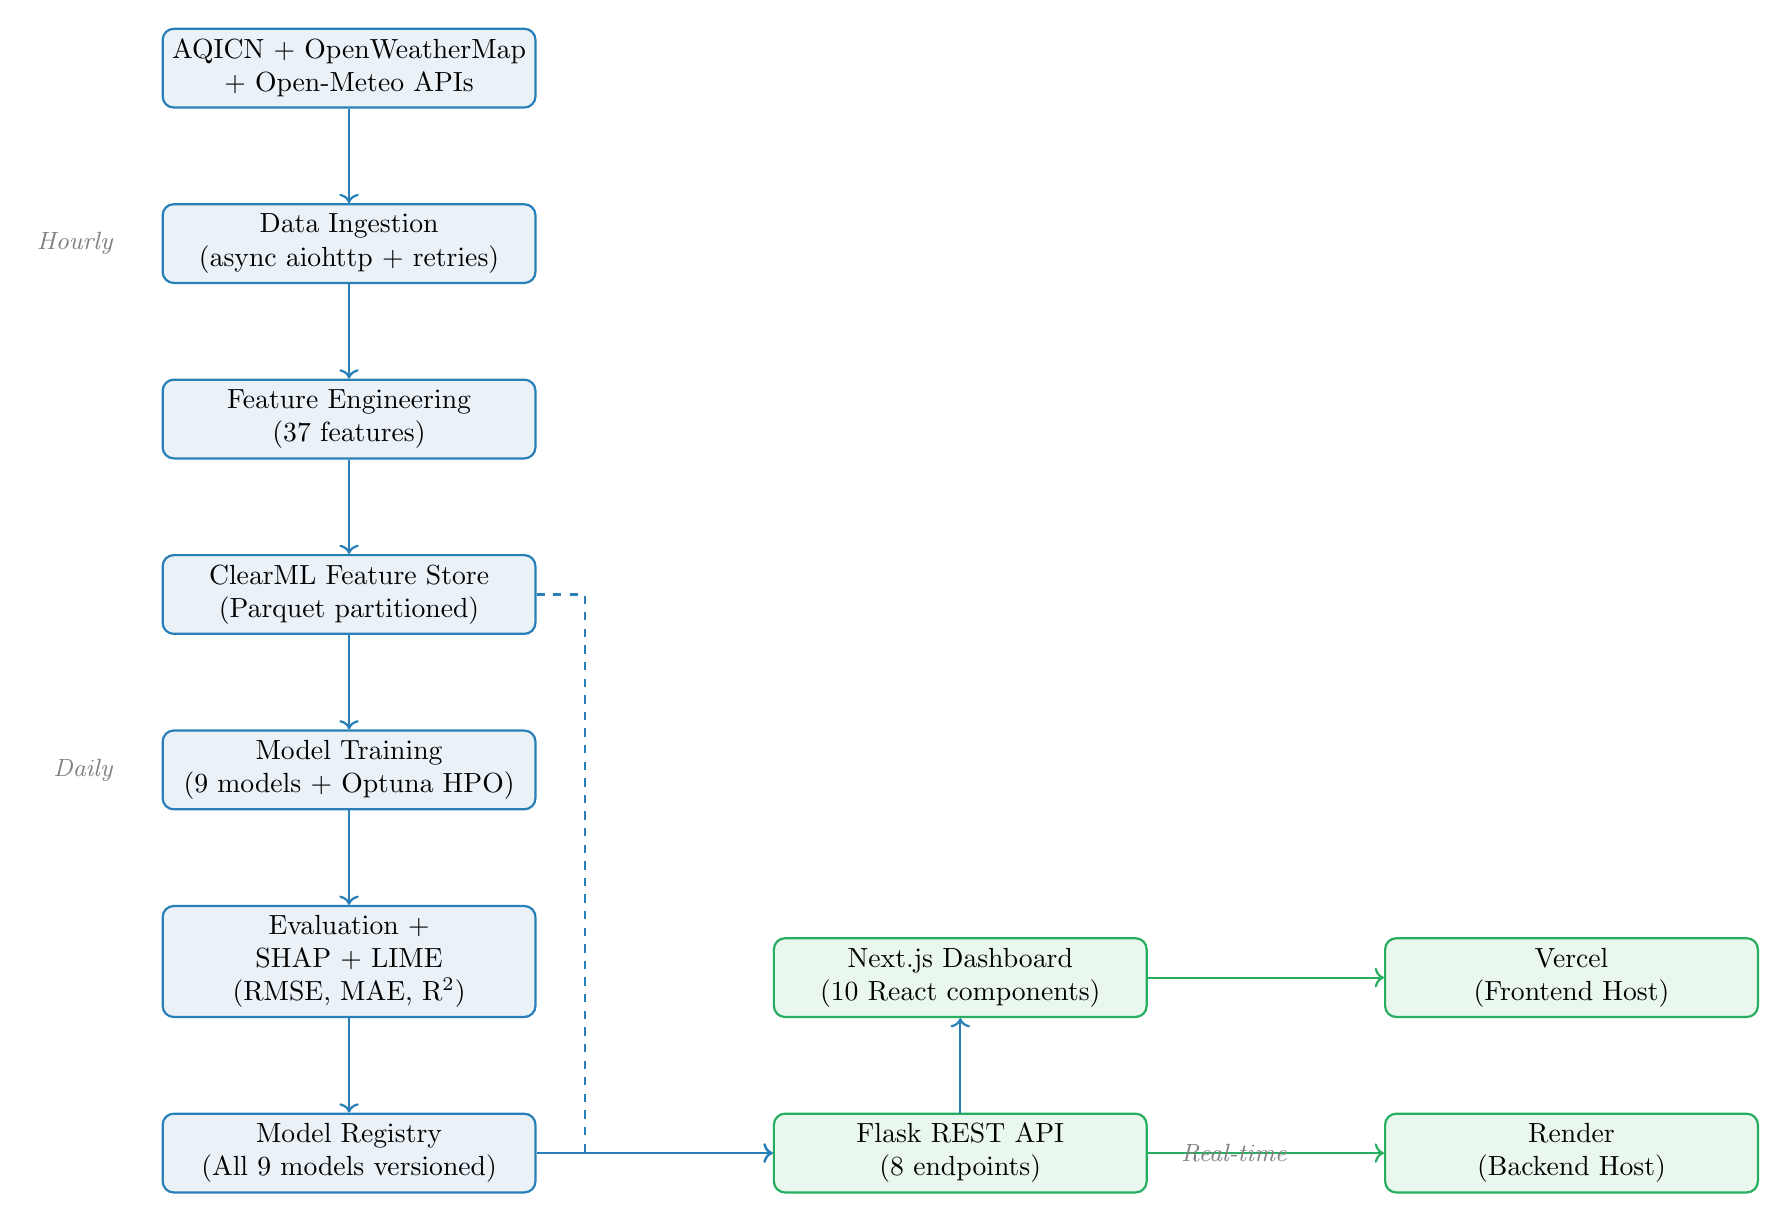
\begin{tikzpicture}[
    node distance=1.2cm,
    block/.style={rectangle, draw=primaryblue, thick, fill=primaryblue!10, text width=4.5cm, text centered, rounded corners, minimum height=1cm},
    deploy/.style={rectangle, draw=accentgreen, thick, fill=accentgreen!10, text width=4.5cm, text centered, rounded corners, minimum height=1cm},
    arrow/.style={->, thick, primaryblue},
    label/.style={font=\small\itshape, text=gray}
]
    % Data Sources
    \node[block] (apis) {AQICN + OpenWeatherMap\\+ Open-Meteo APIs};
    
    % Feature Pipeline
    \node[block, below=of apis] (ingest) {Data Ingestion\\(async aiohttp + retries)};
    \node[block, below=of ingest] (engineer) {Feature Engineering\\(37 features)};
    \node[block, below=of engineer] (store) {ClearML Feature Store\\(Parquet partitioned)};
    
    % Training Pipeline
    \node[block, below=of store] (train) {Model Training\\(9 models + Optuna HPO)};
    \node[block, below=of train] (eval) {Evaluation + SHAP + LIME\\(RMSE, MAE, R\textsuperscript{2})};
    \node[block, below=of eval] (registry) {Model Registry\\(All 9 models versioned)};
    
    % Serving
    \node[deploy, right=3cm of registry] (flask) {Flask REST API\\(8 endpoints)};
    \node[deploy, above=of flask] (nextjs) {Next.js Dashboard\\(10 React components)};
    
    % Deployment
    \node[deploy, right=3cm of flask] (render) {Render\\(Backend Host)};
    \node[deploy, above=of render] (vercel) {Vercel\\(Frontend Host)};
    
    % Arrows
    \draw[arrow] (apis) -- (ingest);
    \draw[arrow] (ingest) -- (engineer);
    \draw[arrow] (engineer) -- (store);
    \draw[arrow] (store) -- (train);
    \draw[arrow] (train) -- (eval);
    \draw[arrow] (eval) -- (registry);
    \draw[arrow] (registry) -- (flask);
    \draw[arrow] (flask) -- (nextjs);
    \draw[arrow, dashed] (store) -- ++(3,0) |- (flask);
    \draw[arrow, accentgreen] (flask) -- (render);
    \draw[arrow, accentgreen] (nextjs) -- (vercel);
    
    % Labels
    \node[label, left=0.5cm of ingest] {Hourly};
    \node[label, left=0.5cm of train] {Daily};
    \node[label, right=0.3cm of flask] {Real-time};
\end{tikzpicture}
\caption{System Architecture Overview}
\label{fig:architecture}
\end{figure}

\section{Pipeline Components}

\subsection{Feature Pipeline (Hourly)}
\begin{itemize}
    \item \textbf{Trigger:} GitHub Actions cron (every hour) or manual dispatch
    \item \textbf{Process:} Fetch $\rightarrow$ Validate $\rightarrow$ Transform $\rightarrow$ Store
    \item \textbf{Output:} 37 engineered features pushed to ClearML Dataset
\end{itemize}

\subsection{Training Pipeline (Daily)}
\begin{itemize}
    \item \textbf{Trigger:} GitHub Actions cron (2:00 AM UTC) or manual dispatch
    \item \textbf{Process:} Extract $\rightarrow$ Train 9 Models $\rightarrow$ Evaluate $\rightarrow$ SHAP/LIME $\rightarrow$ Register All
    \item \textbf{Output:} All 9 trained models registered in ClearML and saved to a local manifest (\texttt{model\_registry.json})
\end{itemize}

\subsection{Serving Layer}
\begin{itemize}
    \item \textbf{API:} Flask REST with 8 endpoints (predict, explain, health, historical, models, simulate, satellite, shadow)
    \item \textbf{Frontend:} Next.js dashboard with 10 interactive React components for forecast visualization, model selection, and causal simulation
    \item \textbf{Deployment:} Backend on Render (Python, Gunicorn), Frontend on Vercel (Next.js, CDN-cached)
\end{itemize}

% ═══════════════════════════════════════════════════════════════════════════════
\chapter{Data Pipeline}
% ═══════════════════════════════════════════════════════════════════════════════

\section{Data Sources}

\begin{table}[H]
\centering
\caption{External Data Sources}
\label{tab:datasources}
\begin{tabularx}{\textwidth}{l l X}
\toprule
\textbf{Source} & \textbf{Data Type} & \textbf{Variables} \\
\midrule
AQICN API & Pollutants & PM2.5, PM10, NO\textsubscript{2}, SO\textsubscript{2}, CO, O\textsubscript{3}, AQI \\
OpenWeatherMap & Weather & Temperature, humidity, wind, pressure, precipitation \\
Open-Meteo Archive & Historical & Hourly air quality + weather (2022--present) \\
\bottomrule
\end{tabularx}
\end{table}

\section{Historical Data Backfill}

The backfill pipeline fetches \textbf{real historical data} from Open-Meteo's free archive APIs:

\begin{lstlisting}[caption={Historical data fetching from Open-Meteo APIs}]
class RealHistoricalDataFetcher:
    def fetch_all(self, start_date, end_date):
        # Air Quality API (PM2.5, PM10, CO, NO2, SO2, O3, US AQI)
        aq_url = f"https://air-quality-api.open-meteo.com/v1/air-quality"
                 f"?latitude={lat}&longitude={lon}"
                 f"&start_date={start_date}&end_date={end_date}"
                 f"&hourly=pm10,pm2_5,carbon_monoxide,..."
        
        # Weather Archive (temperature, humidity, wind, pressure)
        w_url = f"https://archive-api.open-meteo.com/v1/archive"
                f"?latitude={lat}&longitude={lon}"
                f"&start_date={start_date}&end_date={end_date}"
                f"&hourly=temperature_2m,relative_humidity_2m,..."
\end{lstlisting}

Features of the backfill pipeline:
\begin{itemize}
    \item Fetches real hourly observations (not synthetic data)
    \item Supports configurable date ranges via CLI arguments
    \item Checkpoint/resume for interrupted operations
    \item Batch processing to prevent memory overflow
    \item Automatic EDA summary logging after completion
\end{itemize}

\section{Feature Engineering}

The feature engineering module computes \textbf{37 features} from raw pollutant and weather data:

\begin{table}[H]
\centering
\caption{Feature Groups (37 Total Features)}
\label{tab:features}
\begin{tabularx}{\textwidth}{l l X}
\toprule
\textbf{Group} & \textbf{Count} & \textbf{Description} \\
\midrule
Cyclical Temporal & 6 & $\sin/\cos$ encoding of hour, day-of-week, month \\
AQI Change Rate & 3 & Rate of change at 1h, 3h, 6h horizons \\
Wind-Pollutant Interaction & 4 & Wind U/V components $\times$ PM2.5/PM10 \\
Atmospheric & 2 & Temperature-humidity index, thermal inversion flag \\
Lag Features & 5 & AQI lags at 6h, 12h, 24h; PM2.5 lags at 1h, 3h \\
Rolling Statistics & 3 & PM2.5 rolling mean/std (6h, 24h windows) \\
Pollution Index & 1 & Composite normalized pollutant intensity \\
Raw Features & 13 & Direct pollutant and weather measurements \\
\bottomrule
\end{tabularx}
\end{table}

\begin{warnbox}[Leakage Prevention]
Short-horizon lags (1h, 3h for AQI) are excluded from training features to prevent information leakage in the 72-hour forecasting context. Only lags $\geq$ 6h are used as model inputs.
\end{warnbox}

% ═══════════════════════════════════════════════════════════════════════════════
\chapter{Exploratory Data Analysis}
% ═══════════════════════════════════════════════════════════════════════════════

\section{Dataset Overview}

\begin{table}[H]
\centering
\caption{Dataset Summary Statistics}
\label{tab:dataset}
\begin{tabular}{lr}
\toprule
\textbf{Metric} & \textbf{Value} \\
\midrule
Total Observations & 43,801 (hourly) \\
Time Span & July 2021 -- July 2026 (5 years) \\
Engineered Features & 47 columns \\
Missing Values & 0 (0.0\%) \\
Mean AQI & 120.0 \\
Median AQI & 119.7 \\
Max AQI Recorded & 279.7 \\
Std Deviation & 60.9 \\
Hazardous Hours (AQI $>$ 150) & 16,085 (36.72\%) \\
\bottomrule
\end{tabular}
\end{table}

\section{AQI Category Distribution}

Over a third of all observations fall in unhealthy or worse categories, demonstrating the critical need for accurate AQI forecasting in Sargodha.

\begin{figure}[H]
\centering
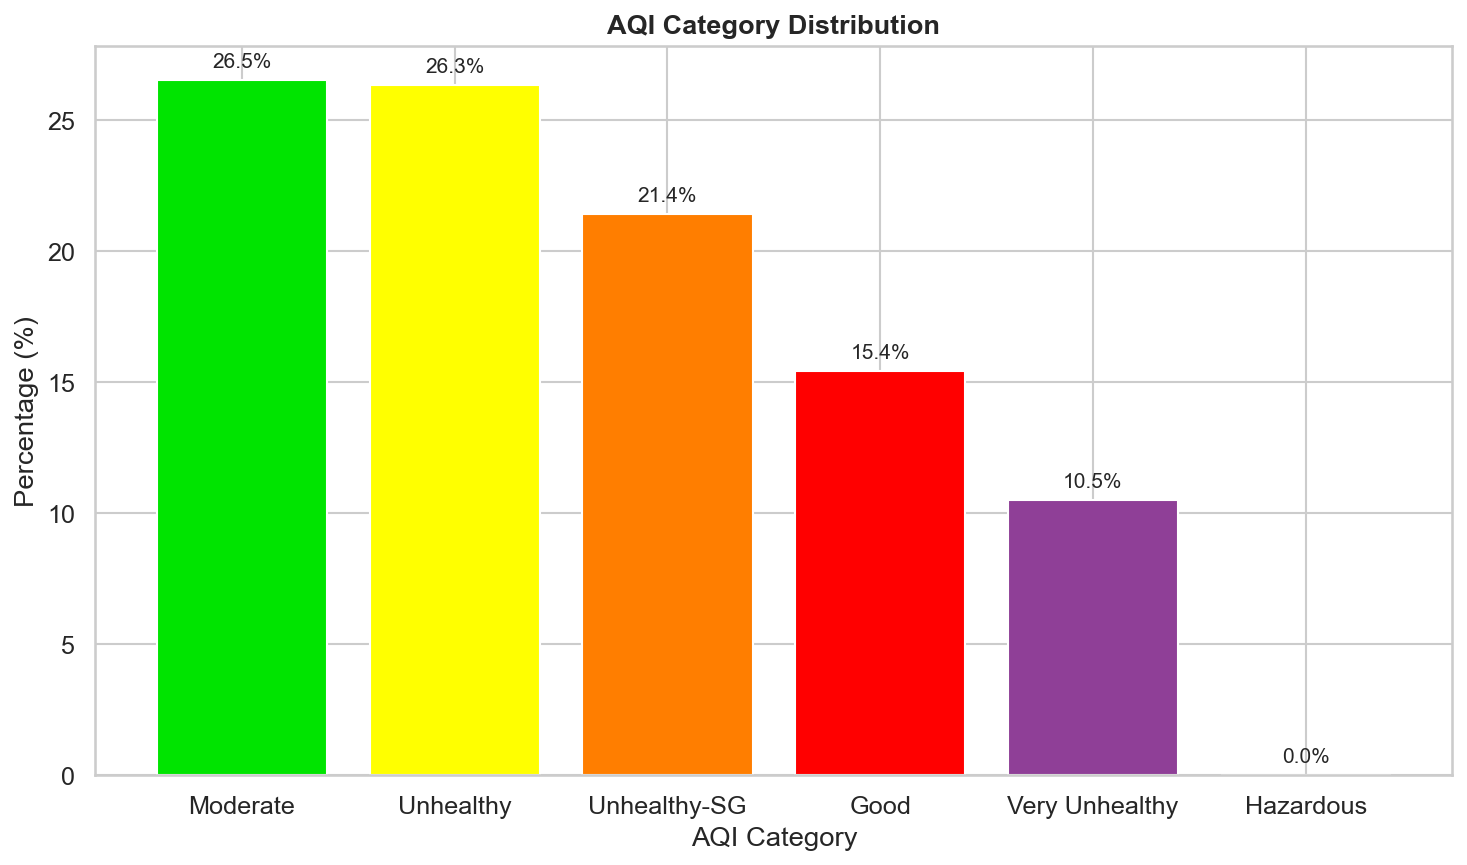
\includegraphics[width=0.85\textwidth]{aqi_category_distribution.png}
\caption{AQI Category Distribution (EPA Standards)}
\label{fig:aqi_categories}
\end{figure}

\section{Pollutant Distributions}

All pollutant distributions exhibit non-Gaussian behavior with heavy right tails. D'Agostino-Pearson normality tests reject normality ($p < 0.001$) for all variables.

\begin{figure}[H]
\centering
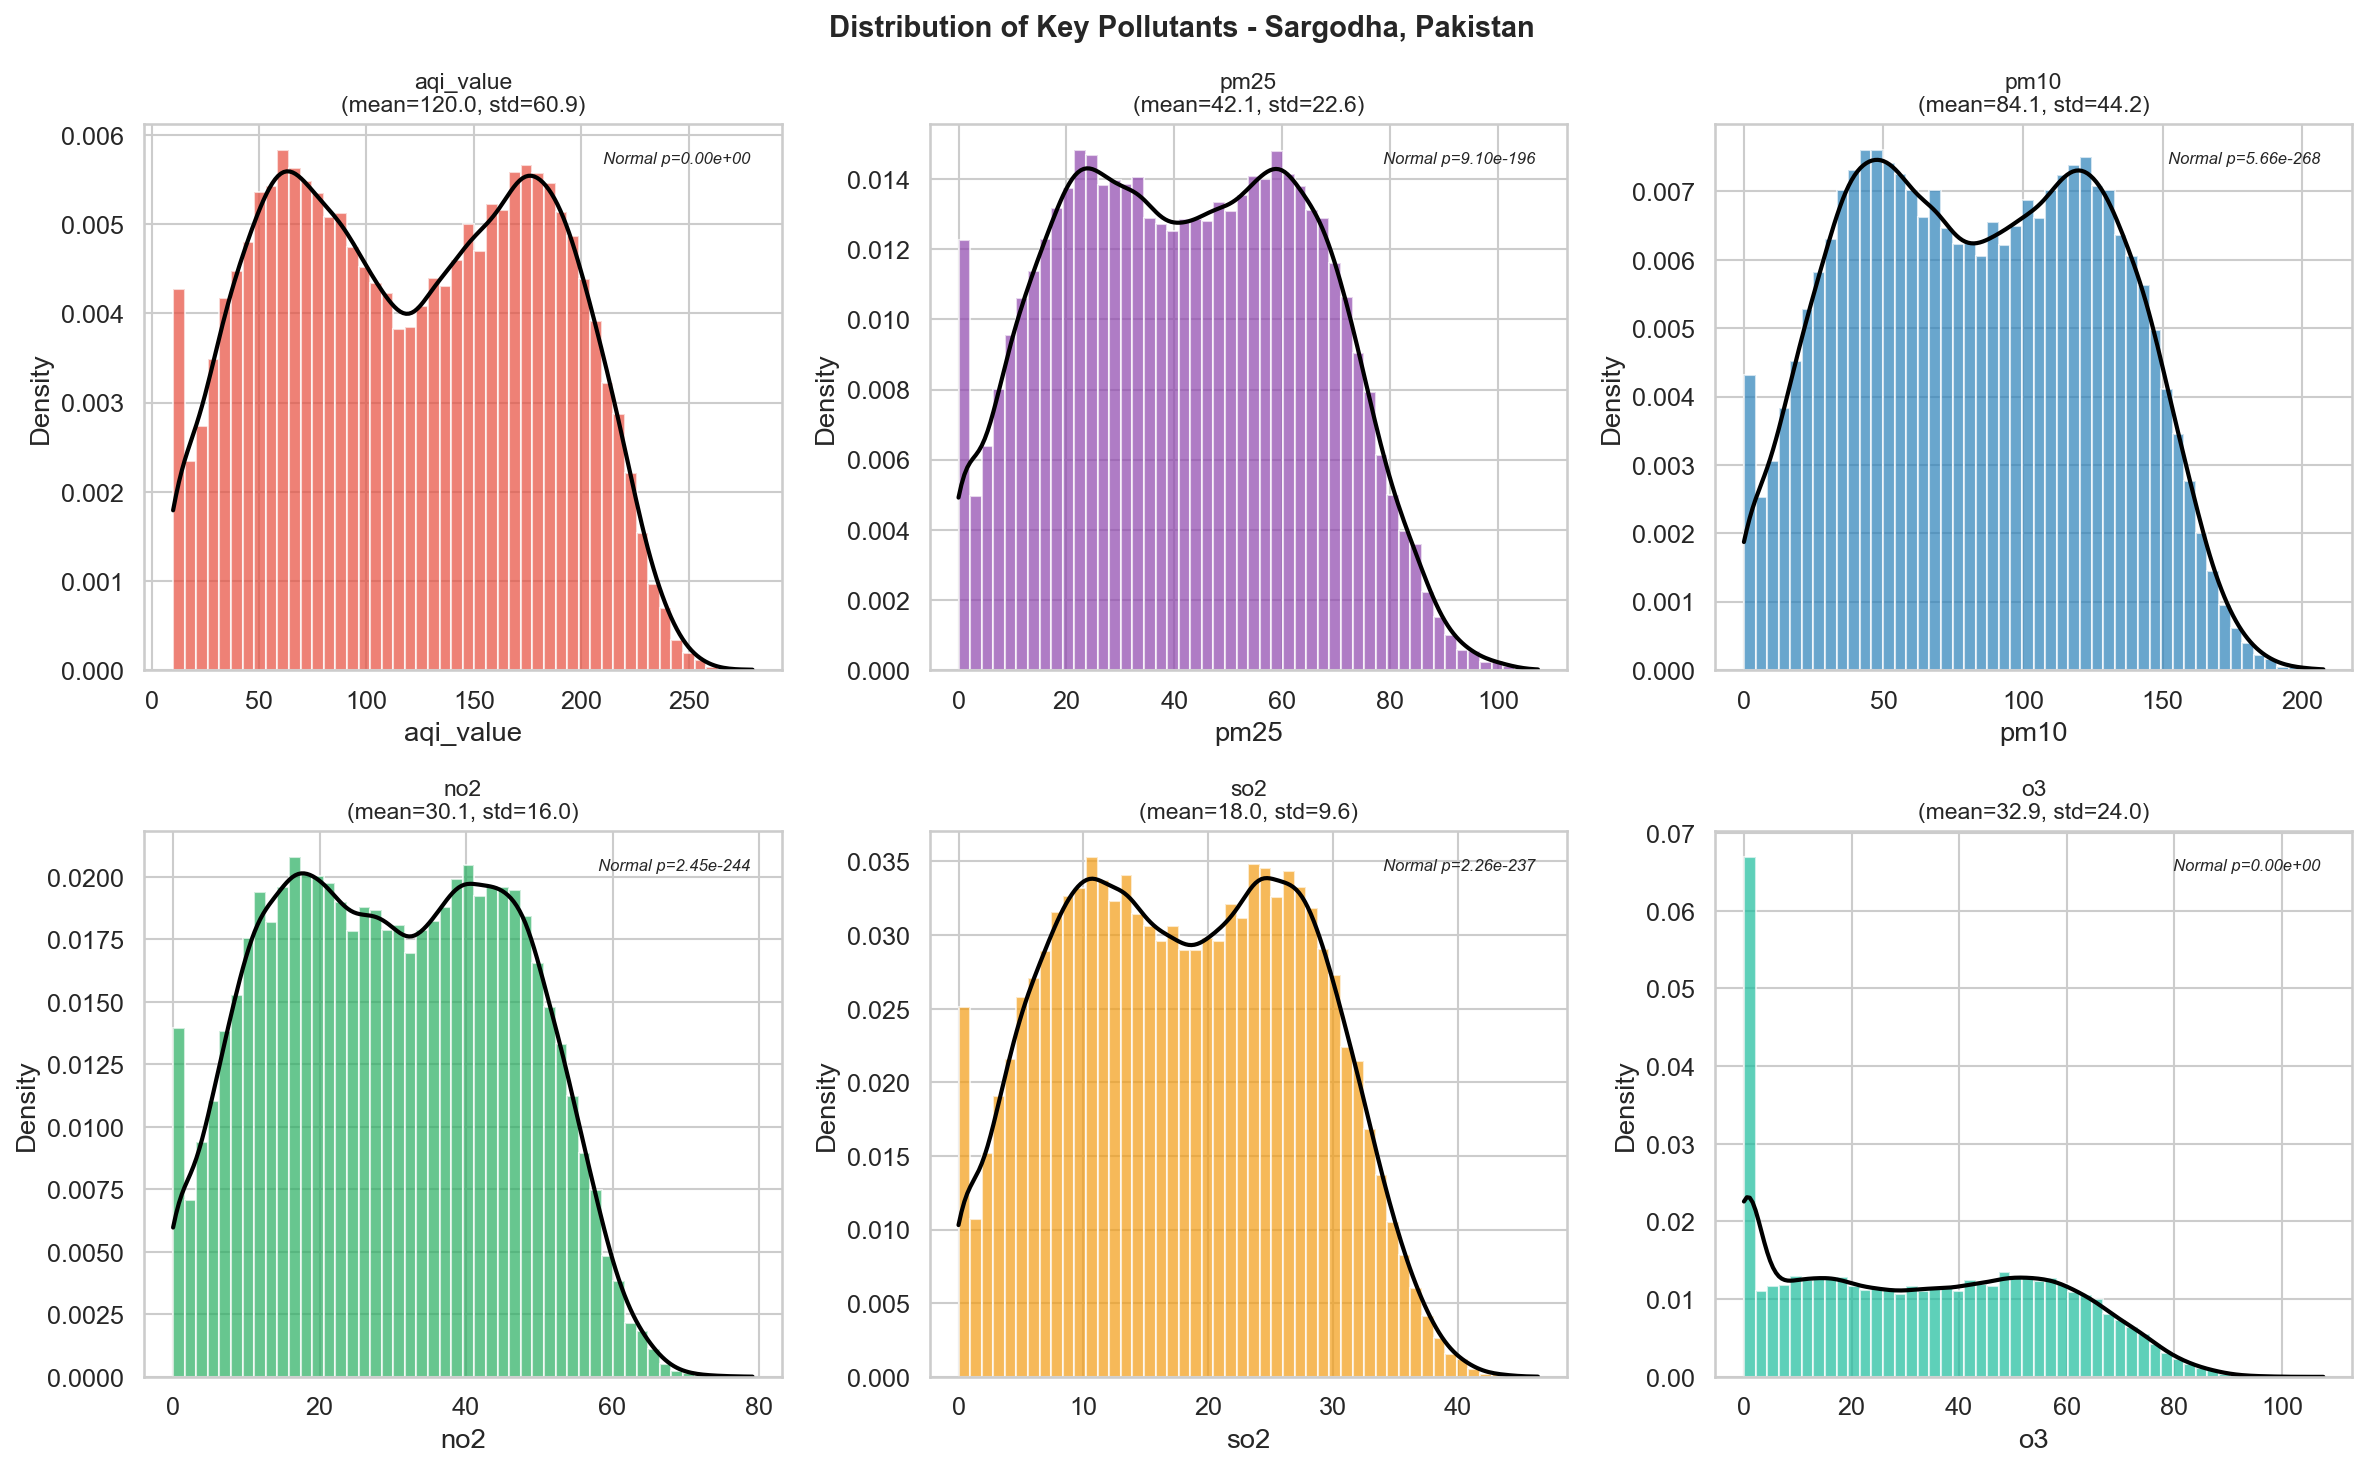
\includegraphics[width=\textwidth]{pollutant_distributions.png}
\caption{Distribution of Key Pollutants with KDE Overlays and Normality Tests}
\label{fig:pollutant_dist}
\end{figure}

\section{Correlation Analysis}

Strong linear relationships exist between AQI and gaseous pollutants (Table~\ref{tab:correlations}).

\begin{figure}[H]
\centering
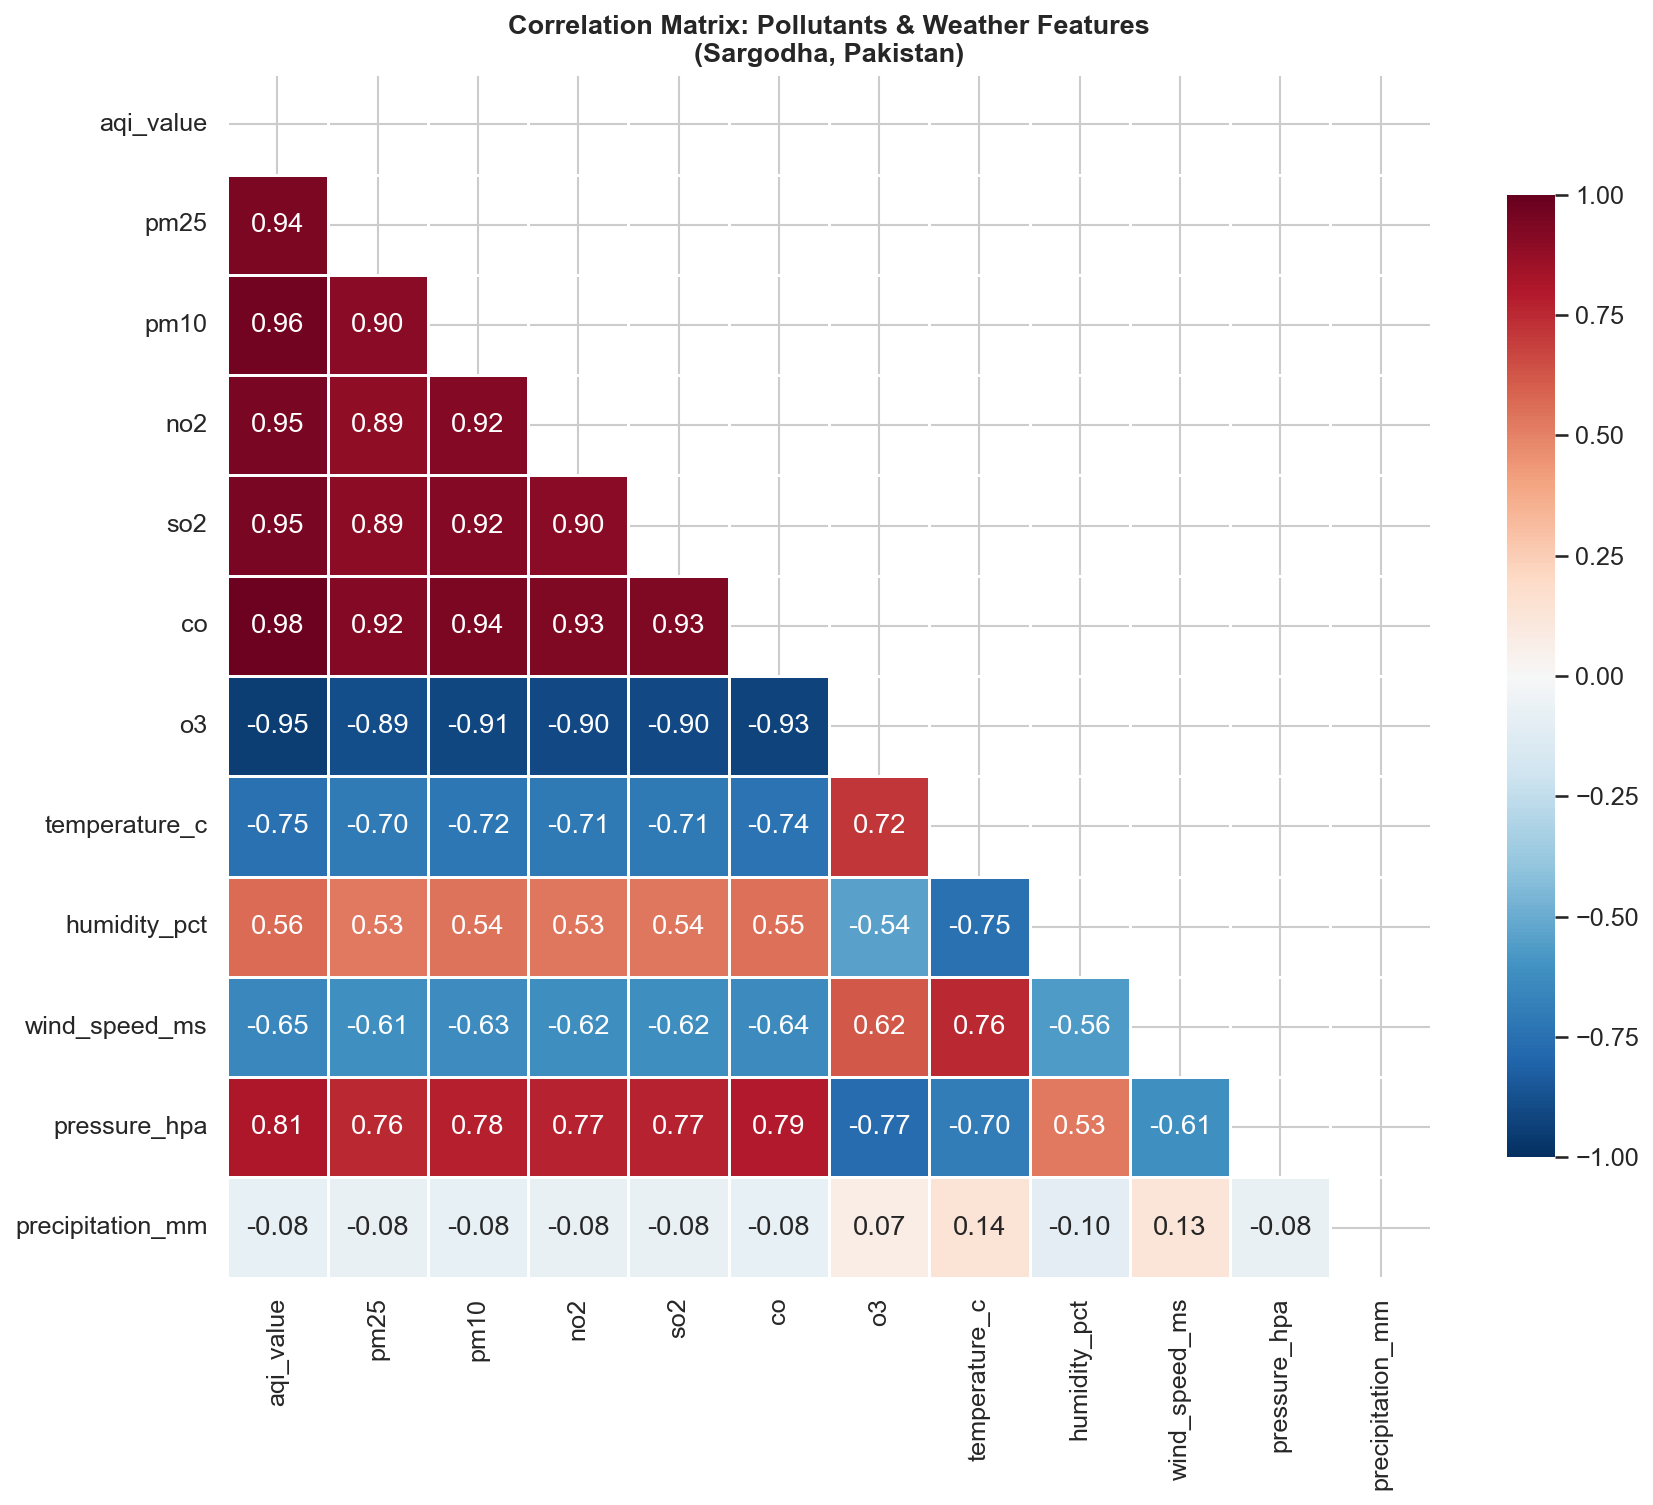
\includegraphics[width=0.9\textwidth]{correlation_heatmap.png}
\caption{Pearson Correlation Matrix: Pollutants and Weather Features}
\label{fig:correlation}
\end{figure}

\begin{table}[H]
\centering
\caption{Top Correlations with AQI (Pearson r)}
\label{tab:correlations}
\begin{tabular}{lr}
\toprule
\textbf{Feature} & \textbf{Correlation} \\
\midrule
CO (Carbon Monoxide) & 0.980 \\
PM10 (Coarse Particulate) & 0.963 \\
NO\textsubscript{2} (Nitrogen Dioxide) & 0.951 \\
SO\textsubscript{2} (Sulfur Dioxide) & 0.951 \\
O\textsubscript{3} (Ozone) & $-0.947$ \\
\bottomrule
\end{tabular}
\end{table}

\begin{figure}[H]
\centering
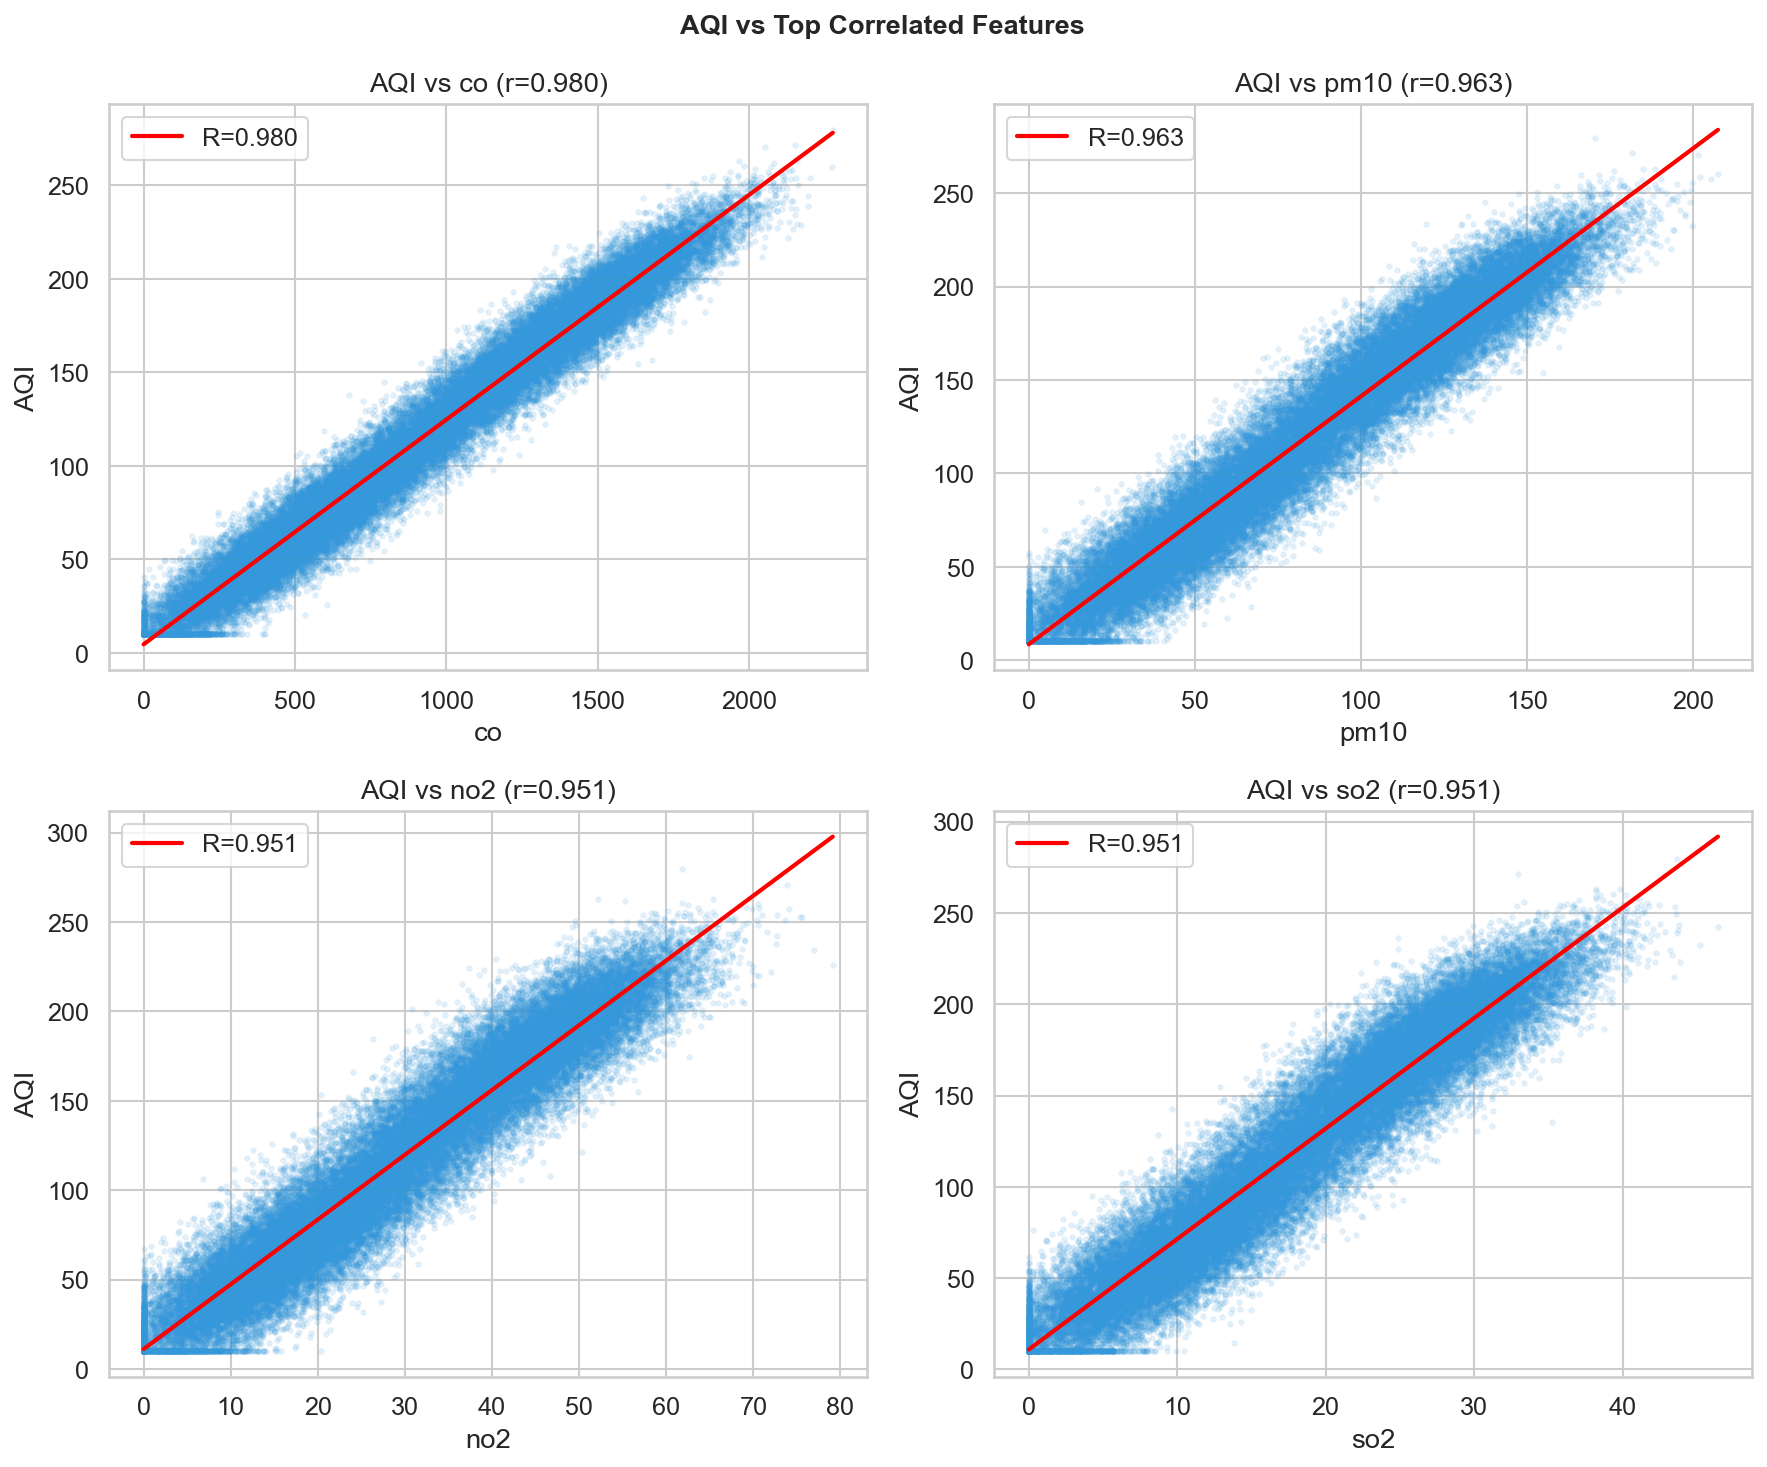
\includegraphics[width=\textwidth]{aqi_scatter_top_features.png}
\caption{AQI vs Top Correlated Features with Regression Lines}
\label{fig:scatter}
\end{figure}

\section{Temporal Patterns}

Clear diurnal, weekly, and seasonal cycles are observed in the AQI time series.

\begin{figure}[H]
\centering
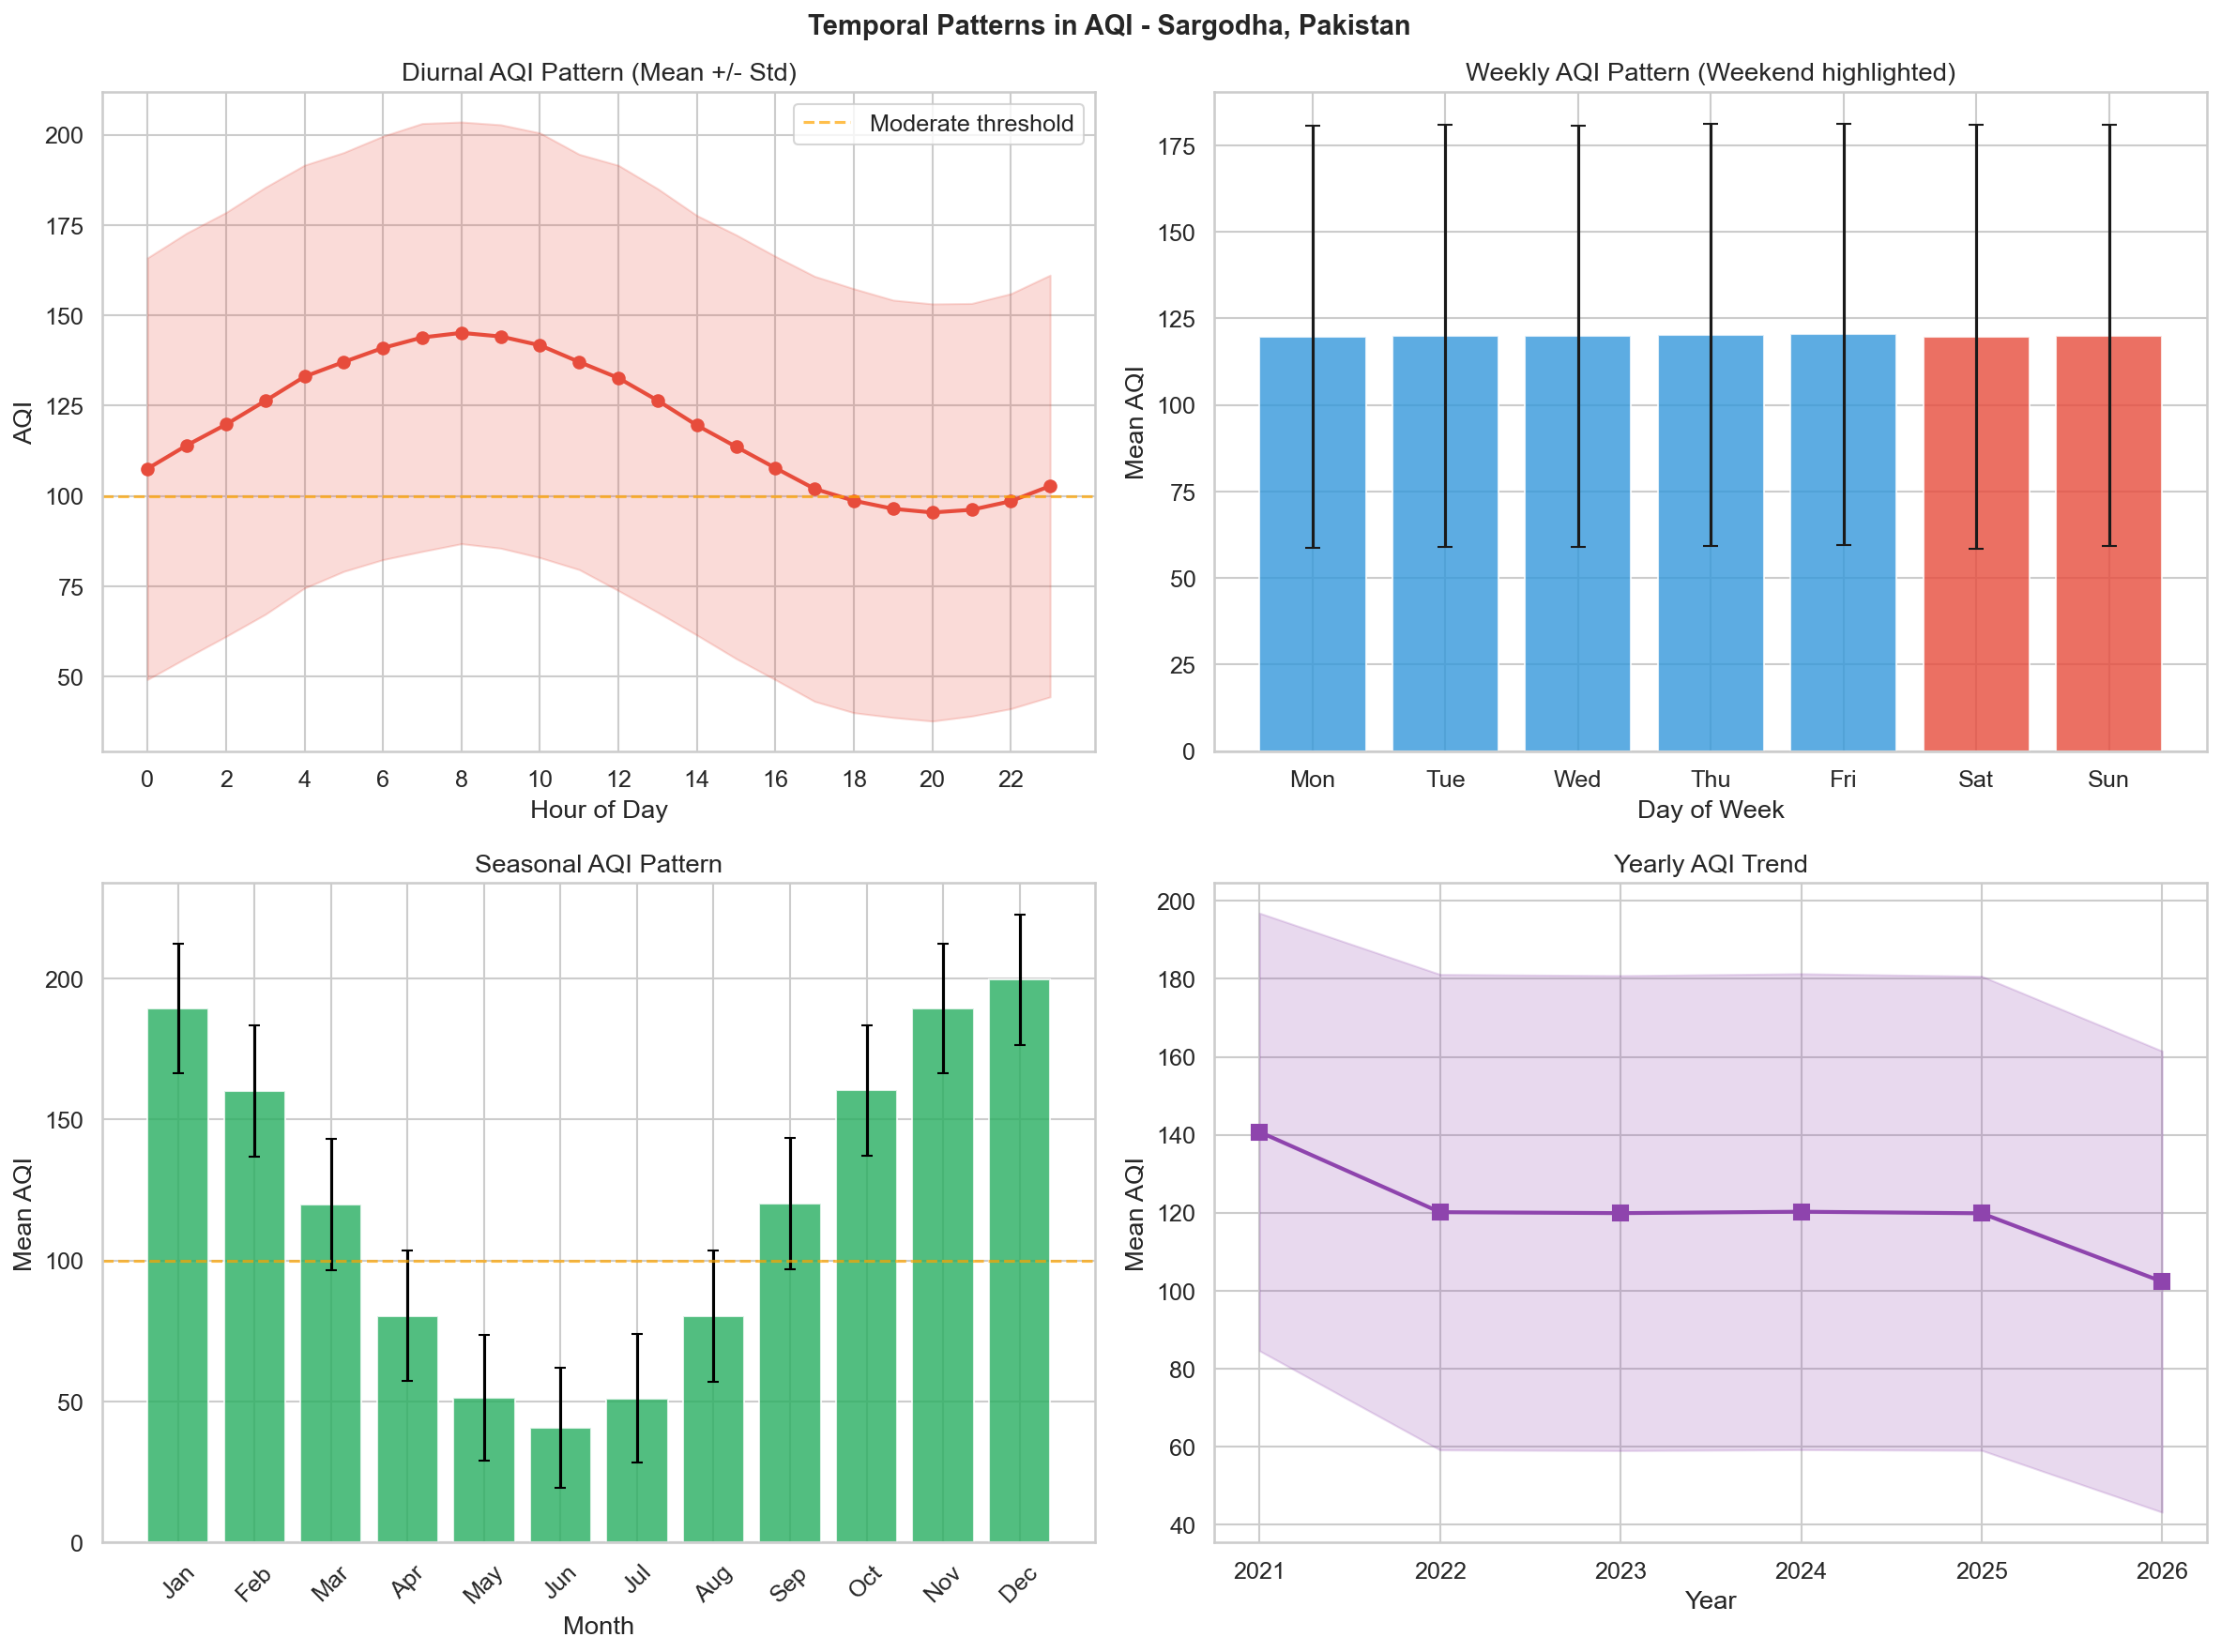
\includegraphics[width=\textwidth]{temporal_patterns.png}
\caption{Temporal AQI Patterns: Diurnal, Weekly, Monthly, and Yearly}
\label{fig:temporal}
\end{figure}

\begin{figure}[H]
\centering
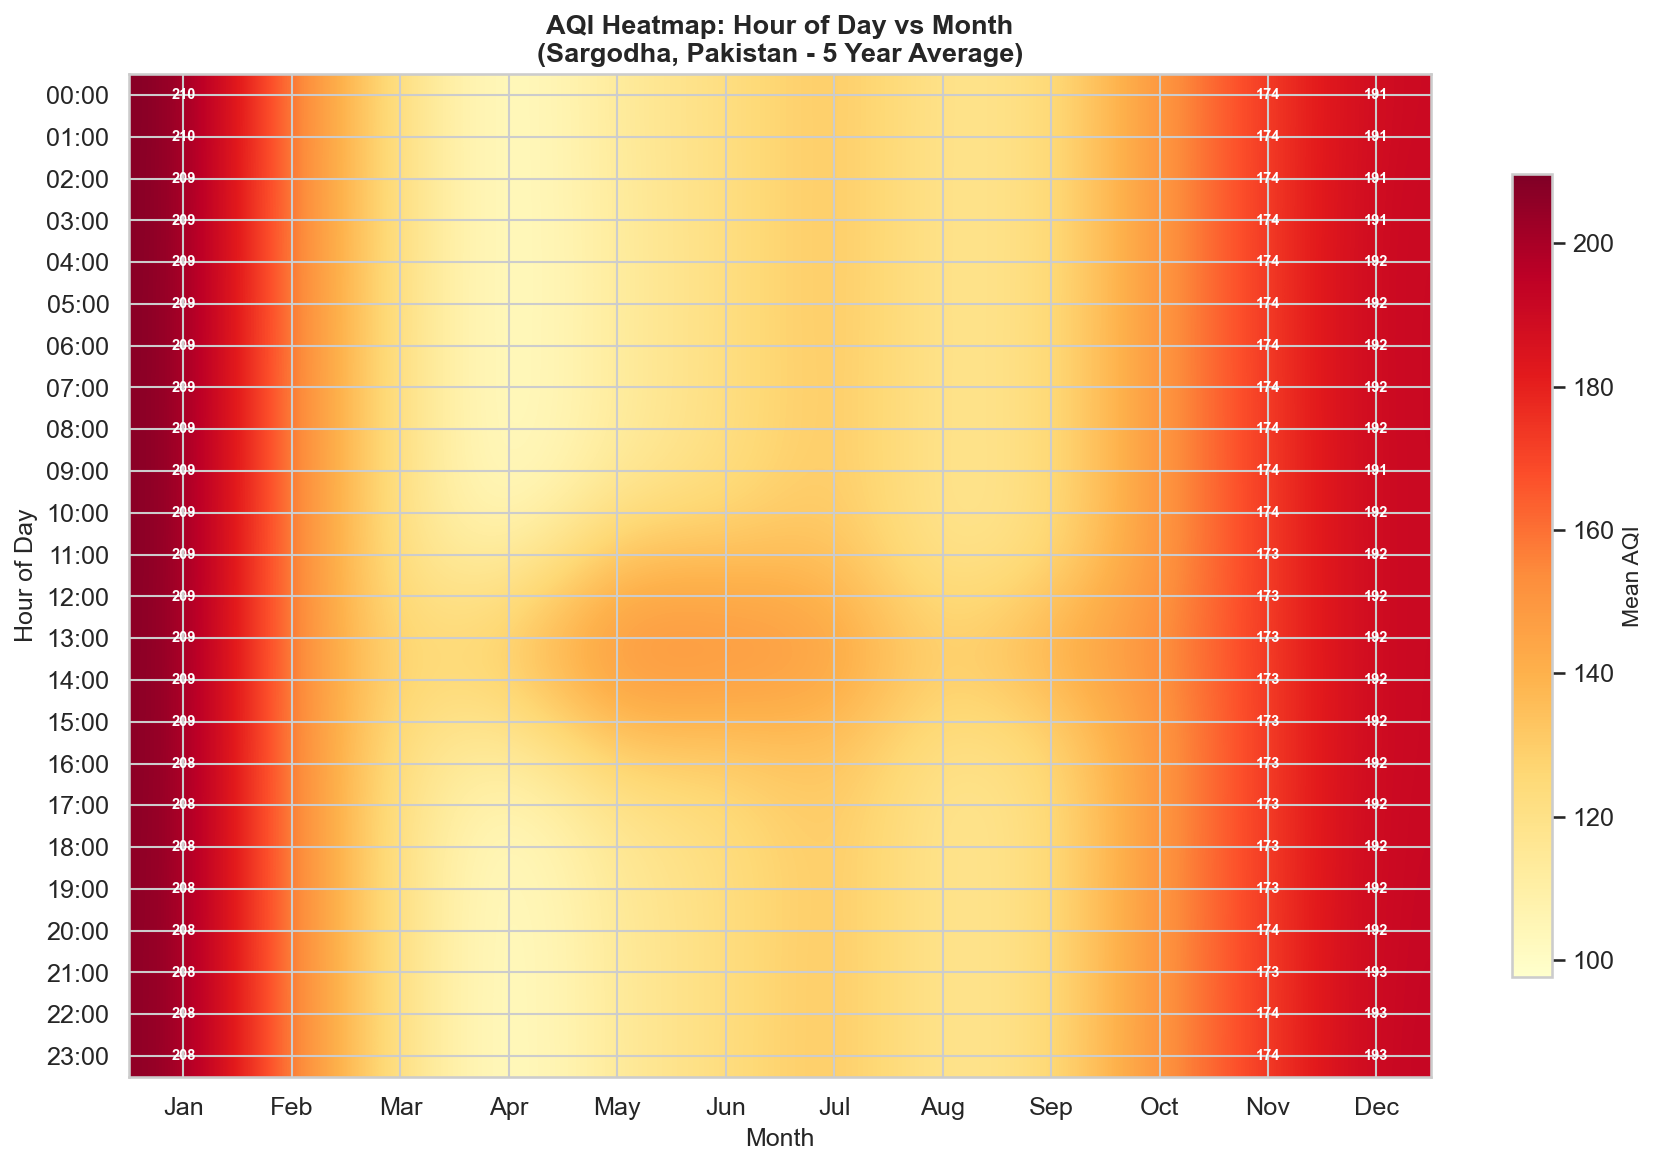
\includegraphics[width=\textwidth]{hour_month_heatmap.png}
\caption{AQI Heatmap: Hour of Day vs Month (Winter Nights are Worst)}
\label{fig:heatmap}
\end{figure}

\section{Time Series Analysis}

\begin{figure}[H]
\centering
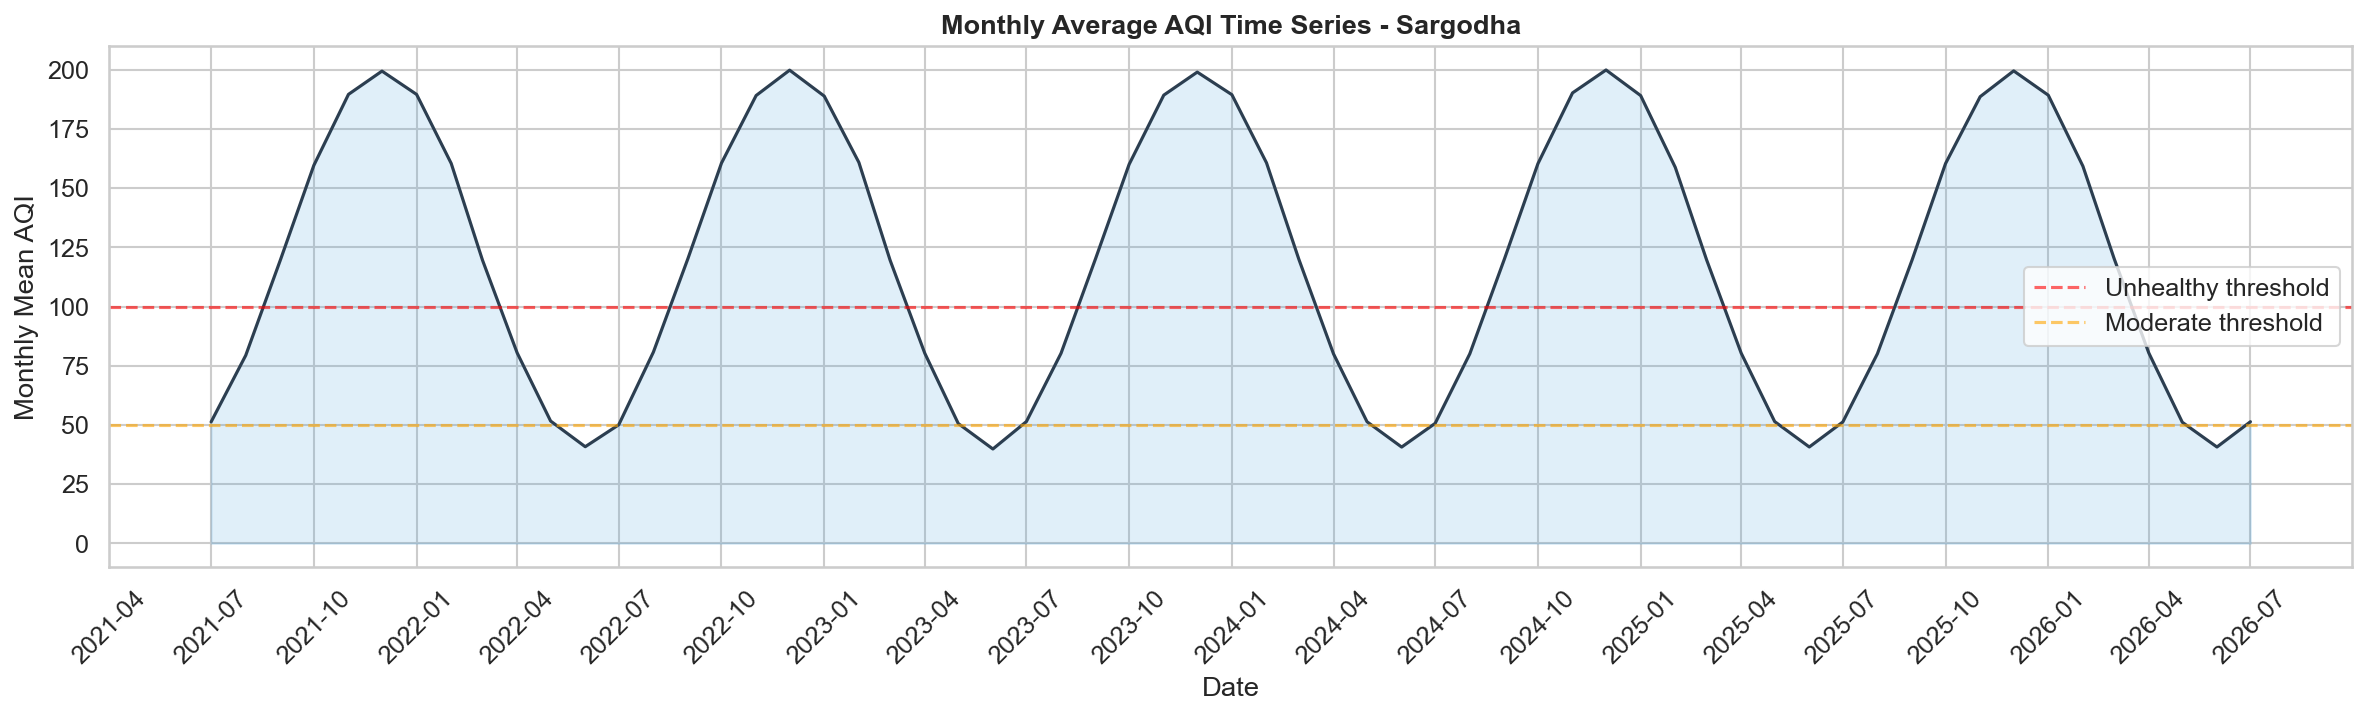
\includegraphics[width=\textwidth]{monthly_aqi_timeseries.png}
\caption{Monthly Average AQI Time Series (5 Years)}
\label{fig:monthly_ts}
\end{figure}

\begin{figure}[H]
\centering
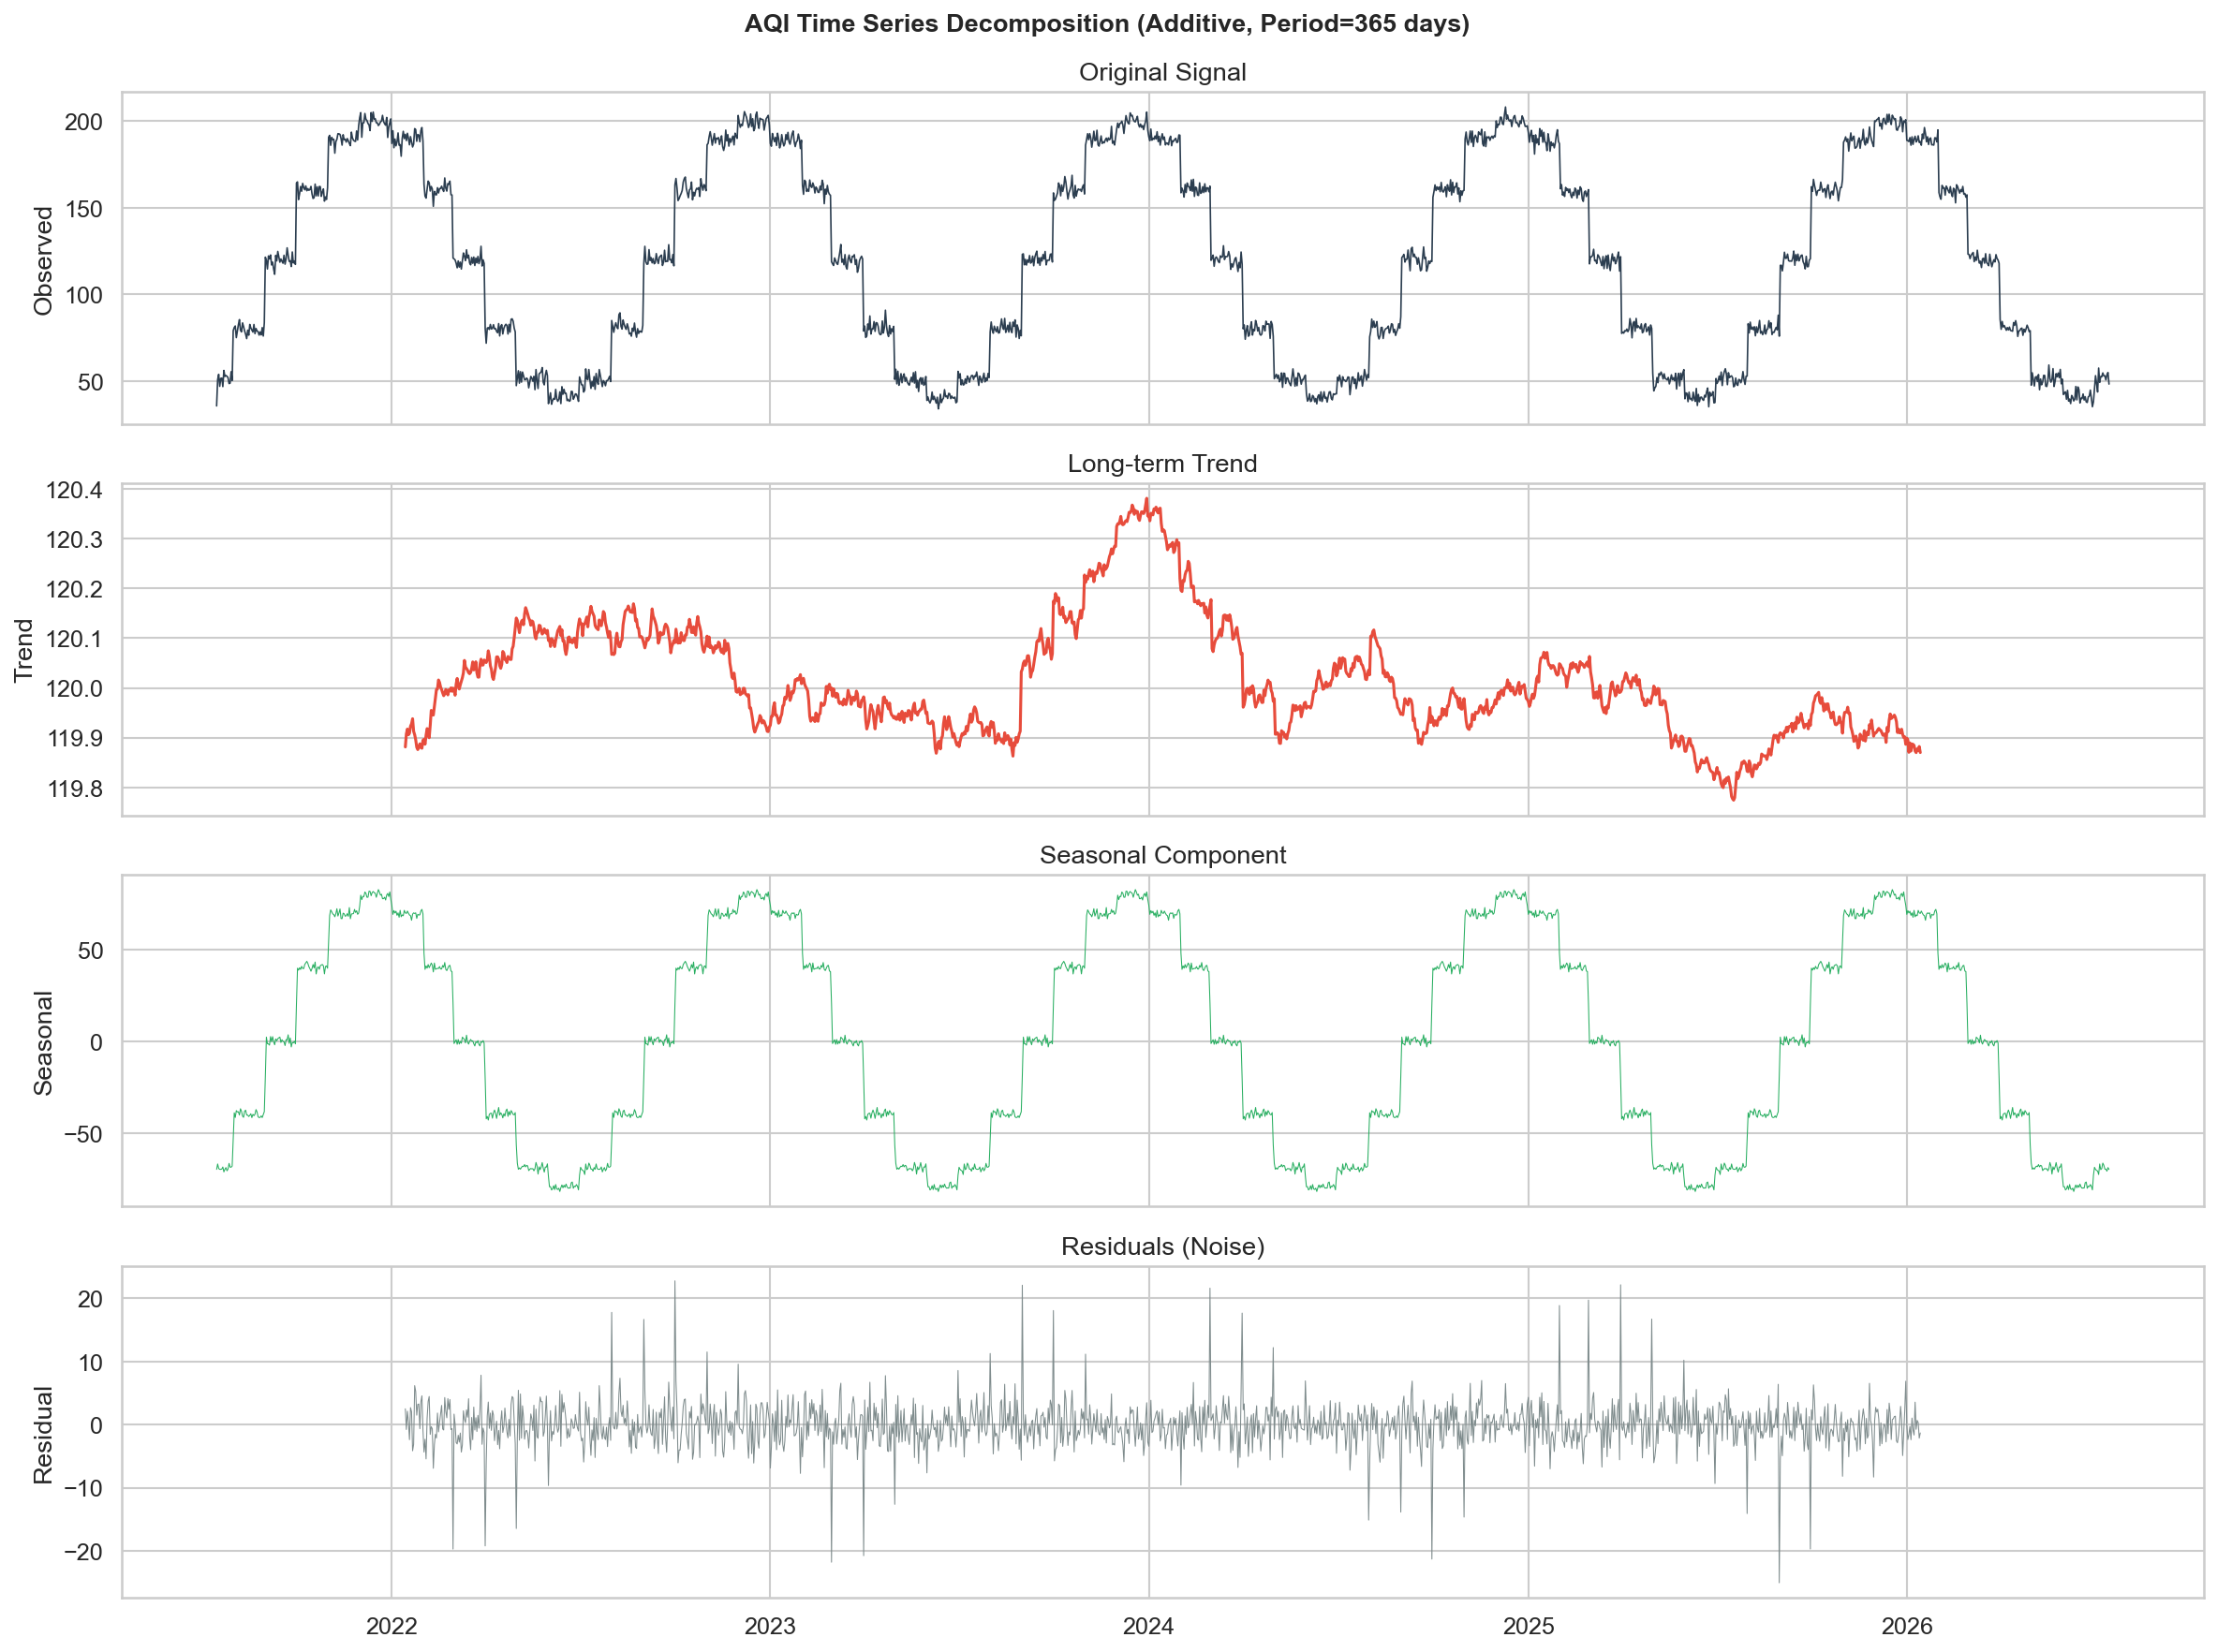
\includegraphics[width=\textwidth]{seasonal_decomposition.png}
\caption{Additive Seasonal Decomposition (Period = 365 Days)}
\label{fig:decomp}
\end{figure}

\subsection{Stationarity Test}

Augmented Dickey-Fuller test on daily-averaged AQI:
\begin{itemize}
    \item ADF Statistic: $-2.12$ (critical value at 5\%: $-2.86$)
    \item $p$-value: $0.237$
    \item \textbf{Conclusion:} Series is non-stationary $\Rightarrow$ lag features and differencing are essential
\end{itemize}

\section{Autocorrelation Analysis}

\begin{figure}[H]
\centering
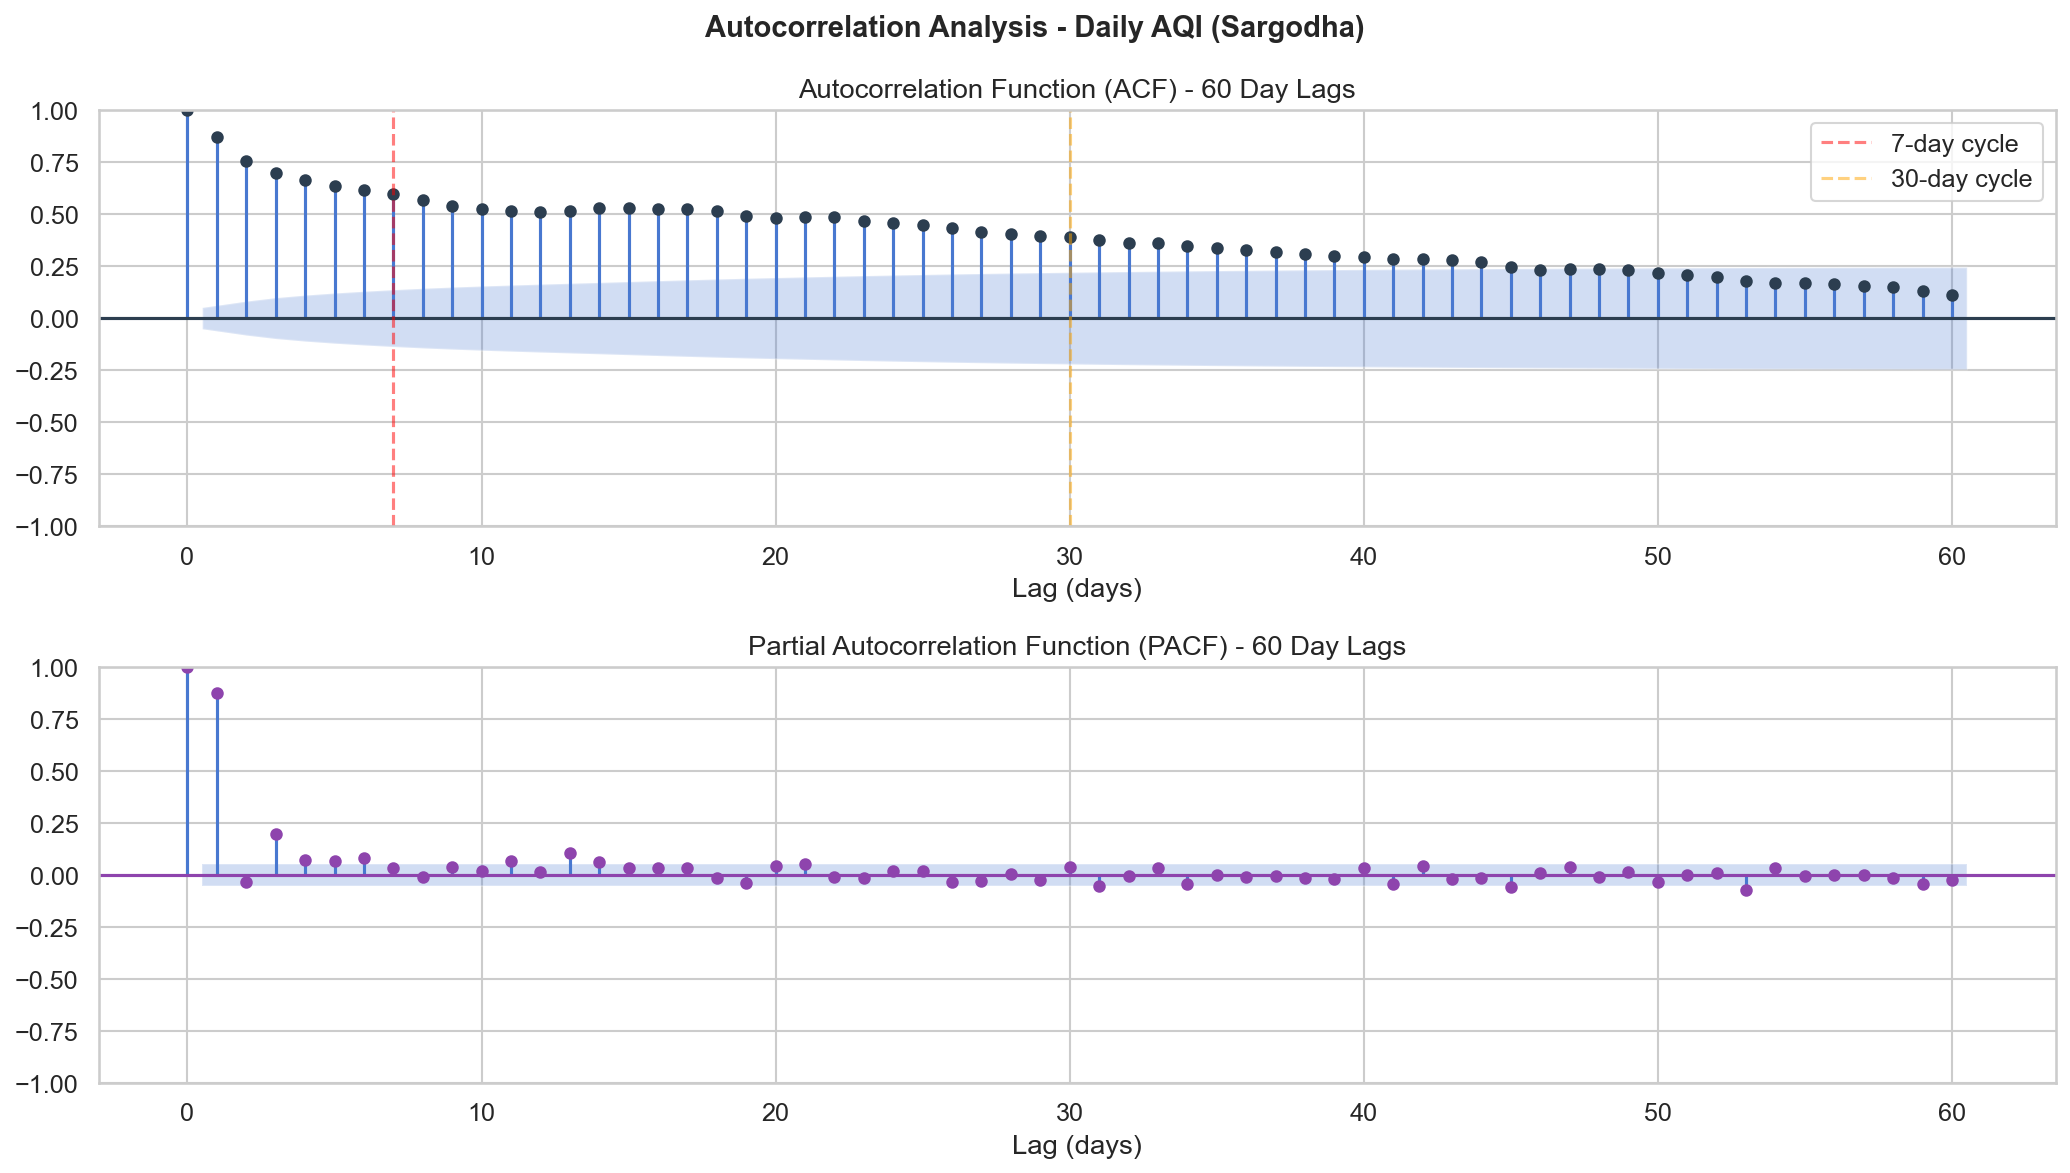
\includegraphics[width=\textwidth]{acf_pacf_analysis.png}
\caption{ACF and PACF of Daily AQI (60-Day Lags)}
\label{fig:acf_pacf}
\end{figure}

\begin{figure}[H]
\centering
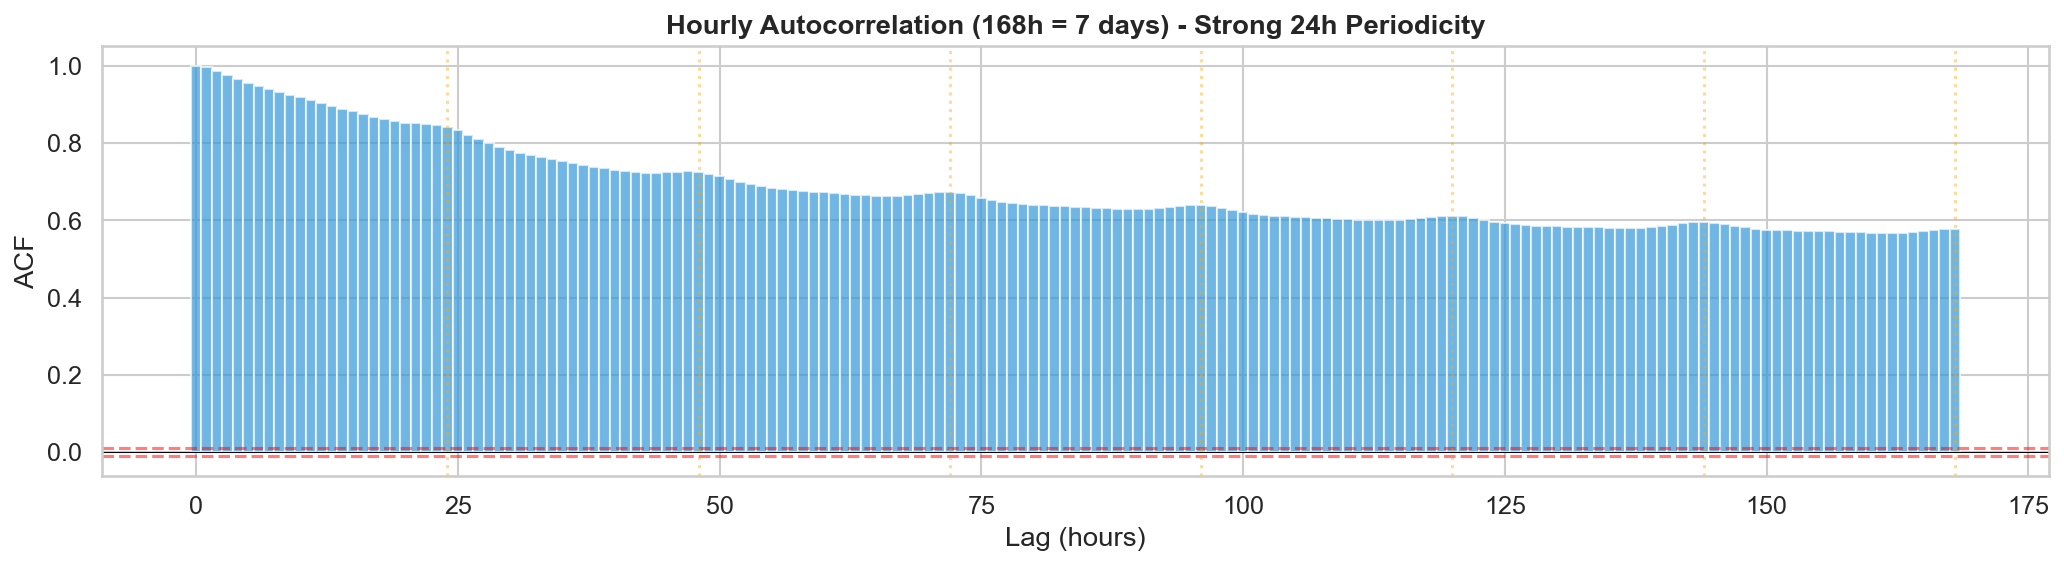
\includegraphics[width=\textwidth]{hourly_acf_168h.png}
\caption{Hourly Autocorrelation Showing Strong 24-Hour Periodicity}
\label{fig:hourly_acf}
\end{figure}

\section{Rolling Volatility}

\begin{figure}[H]
\centering
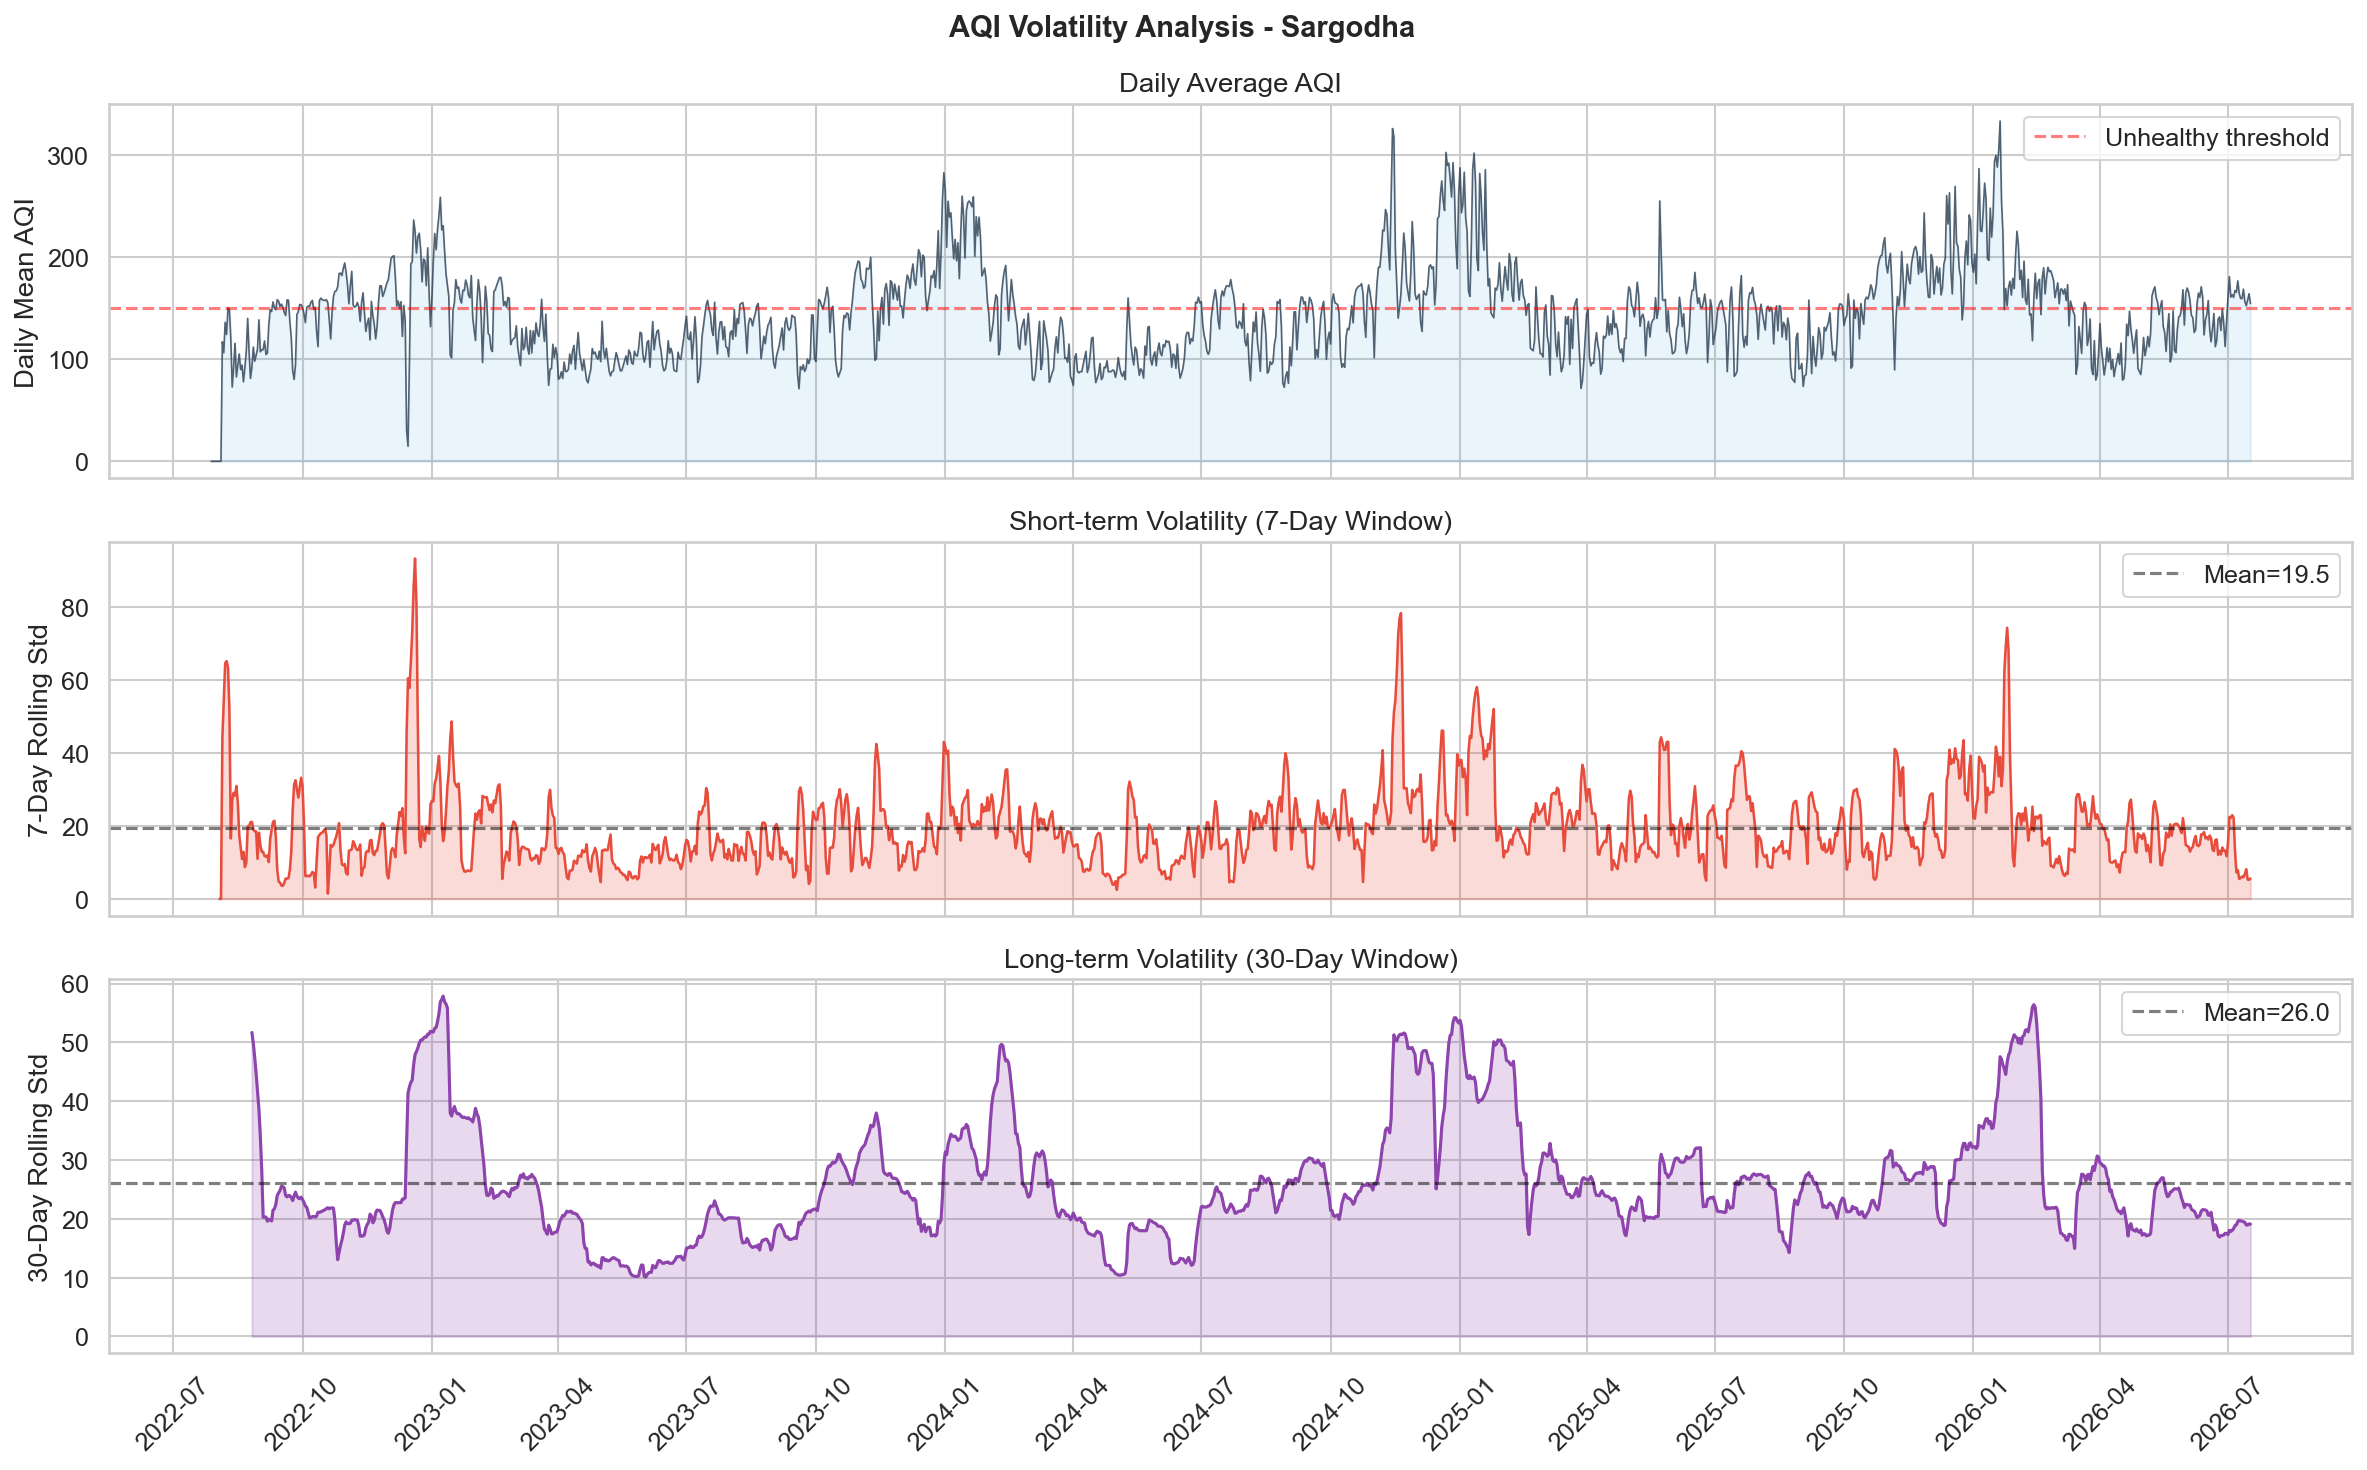
\includegraphics[width=\textwidth]{rolling_volatility.png}
\caption{AQI Volatility: 7-Day and 30-Day Rolling Standard Deviation}
\label{fig:volatility}
\end{figure}

\section{Weather-Pollutant Relationships}

\begin{figure}[H]
\centering
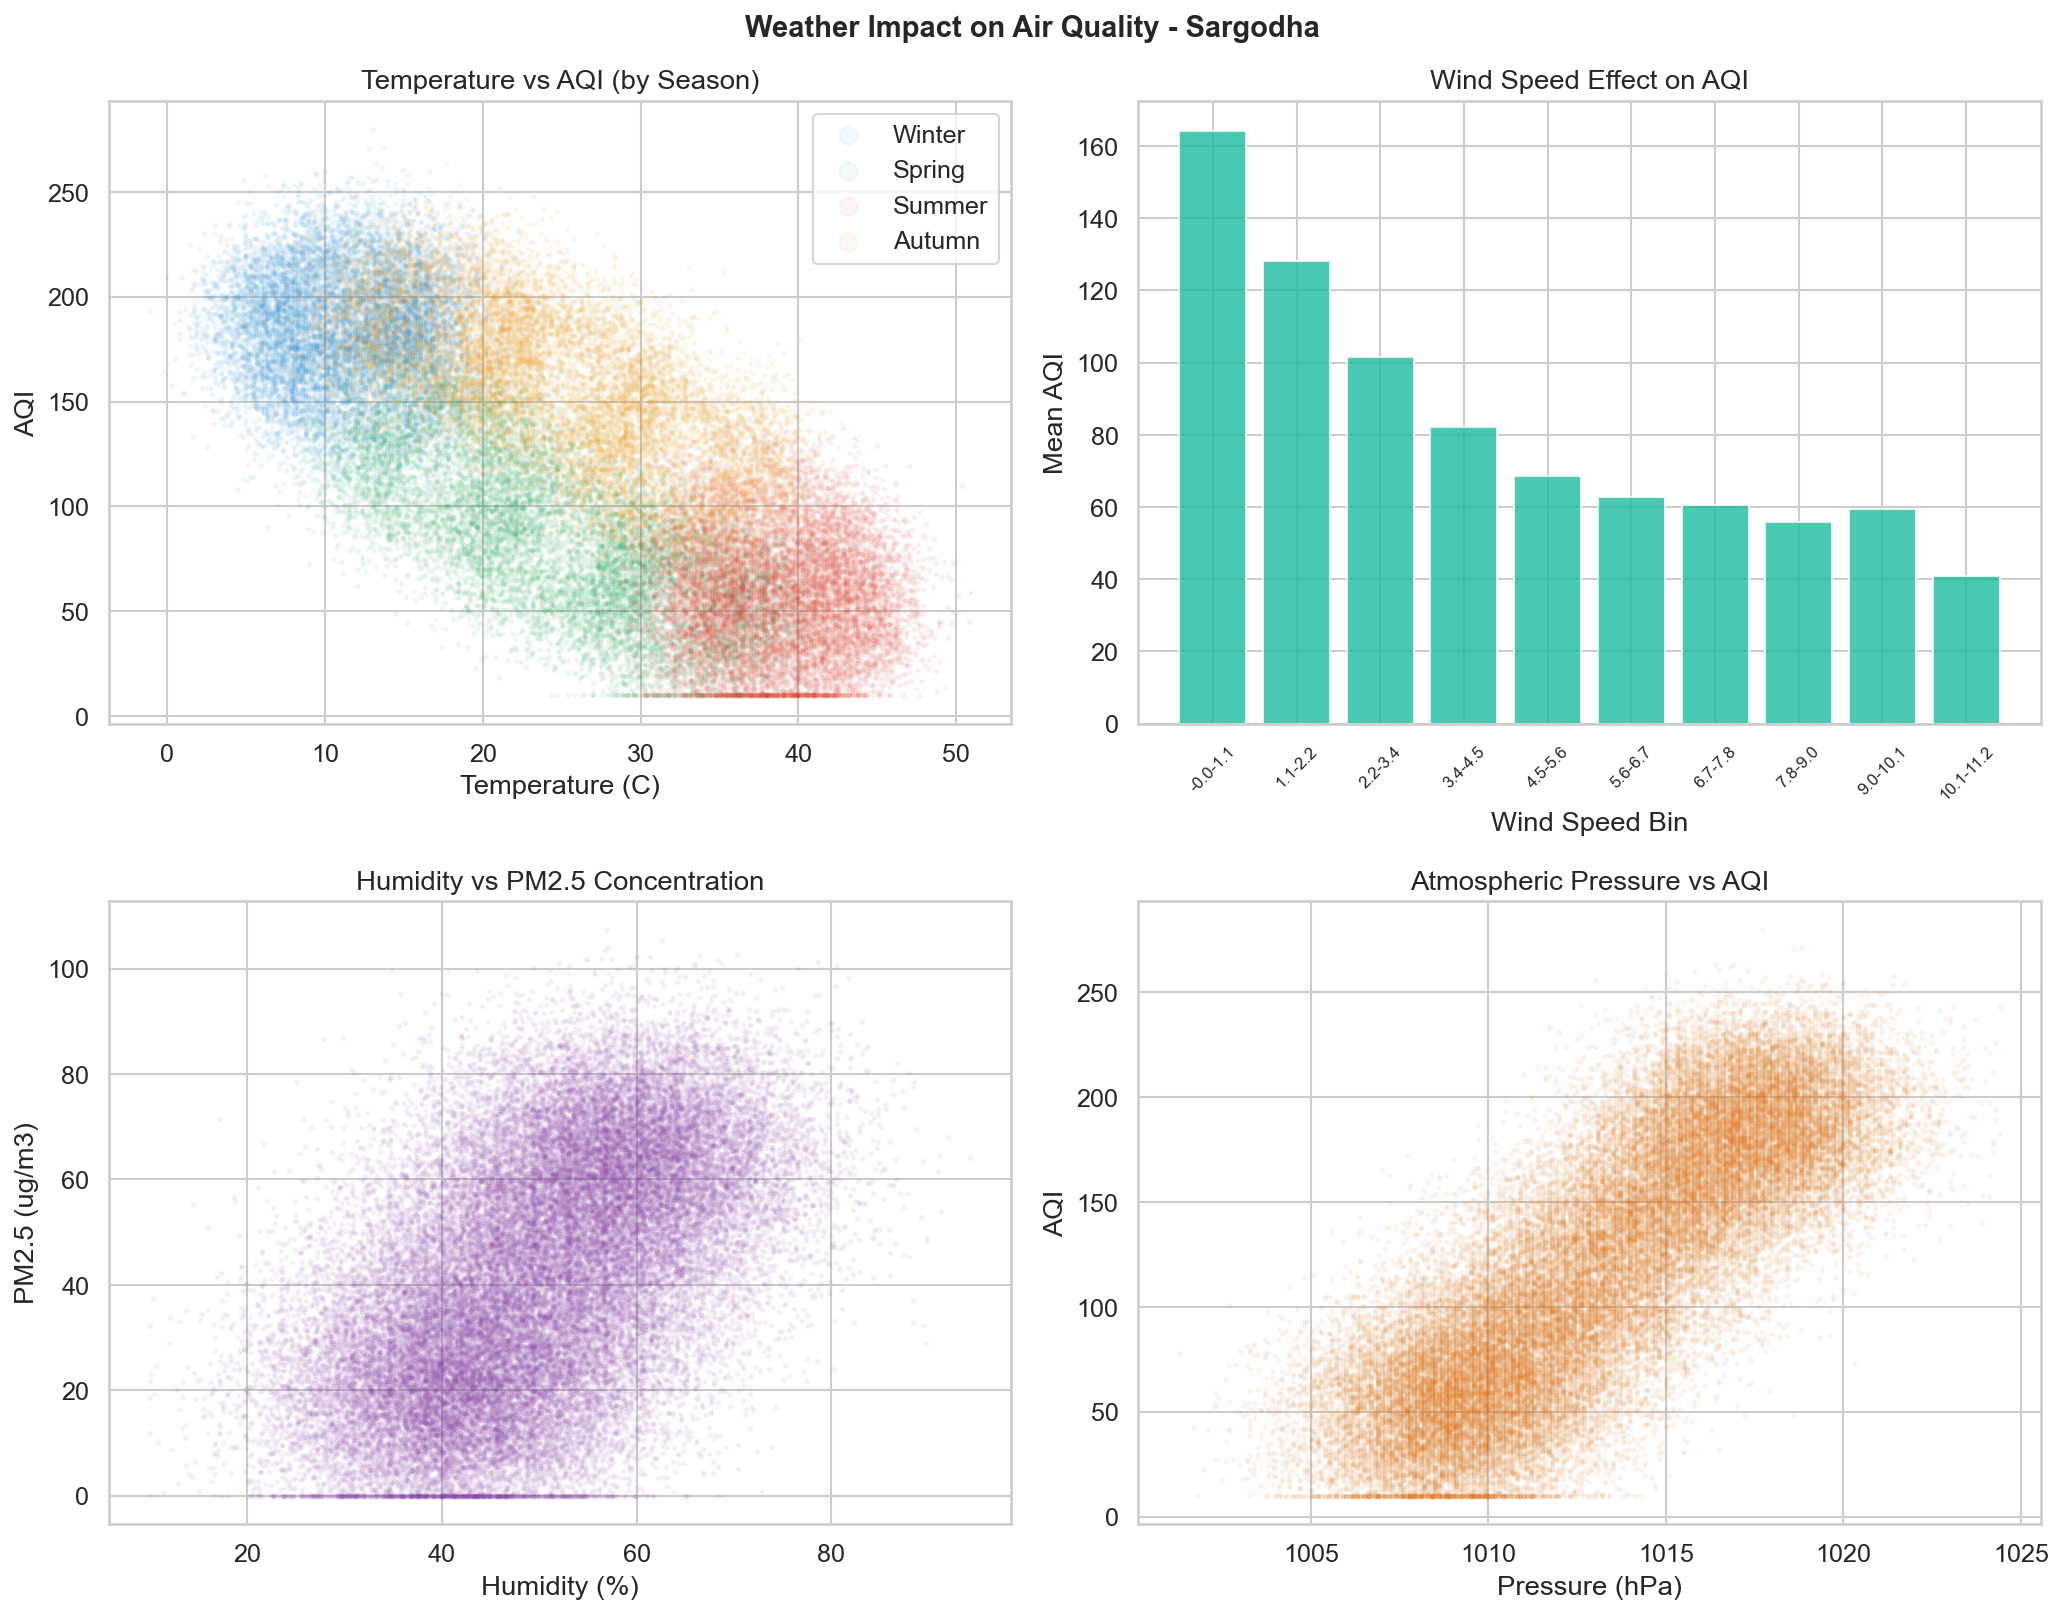
\includegraphics[width=\textwidth]{weather_pollutant_relationships.png}
\caption{Weather Impact on Air Quality (Temperature, Wind, Humidity, Pressure)}
\label{fig:weather}
\end{figure}

\textbf{Hazardous conditions profile} (AQI $>$ 150):
\begin{itemize}
    \item Average temperature: 15.3\textdegree C (cooler months, thermal inversions)
    \item Average humidity: 57.8\%
    \item Average wind speed: 0.8 m/s (near-calm, poor dispersion)
\end{itemize}

\section{Pollution Wind Rose}

\begin{figure}[H]
\centering
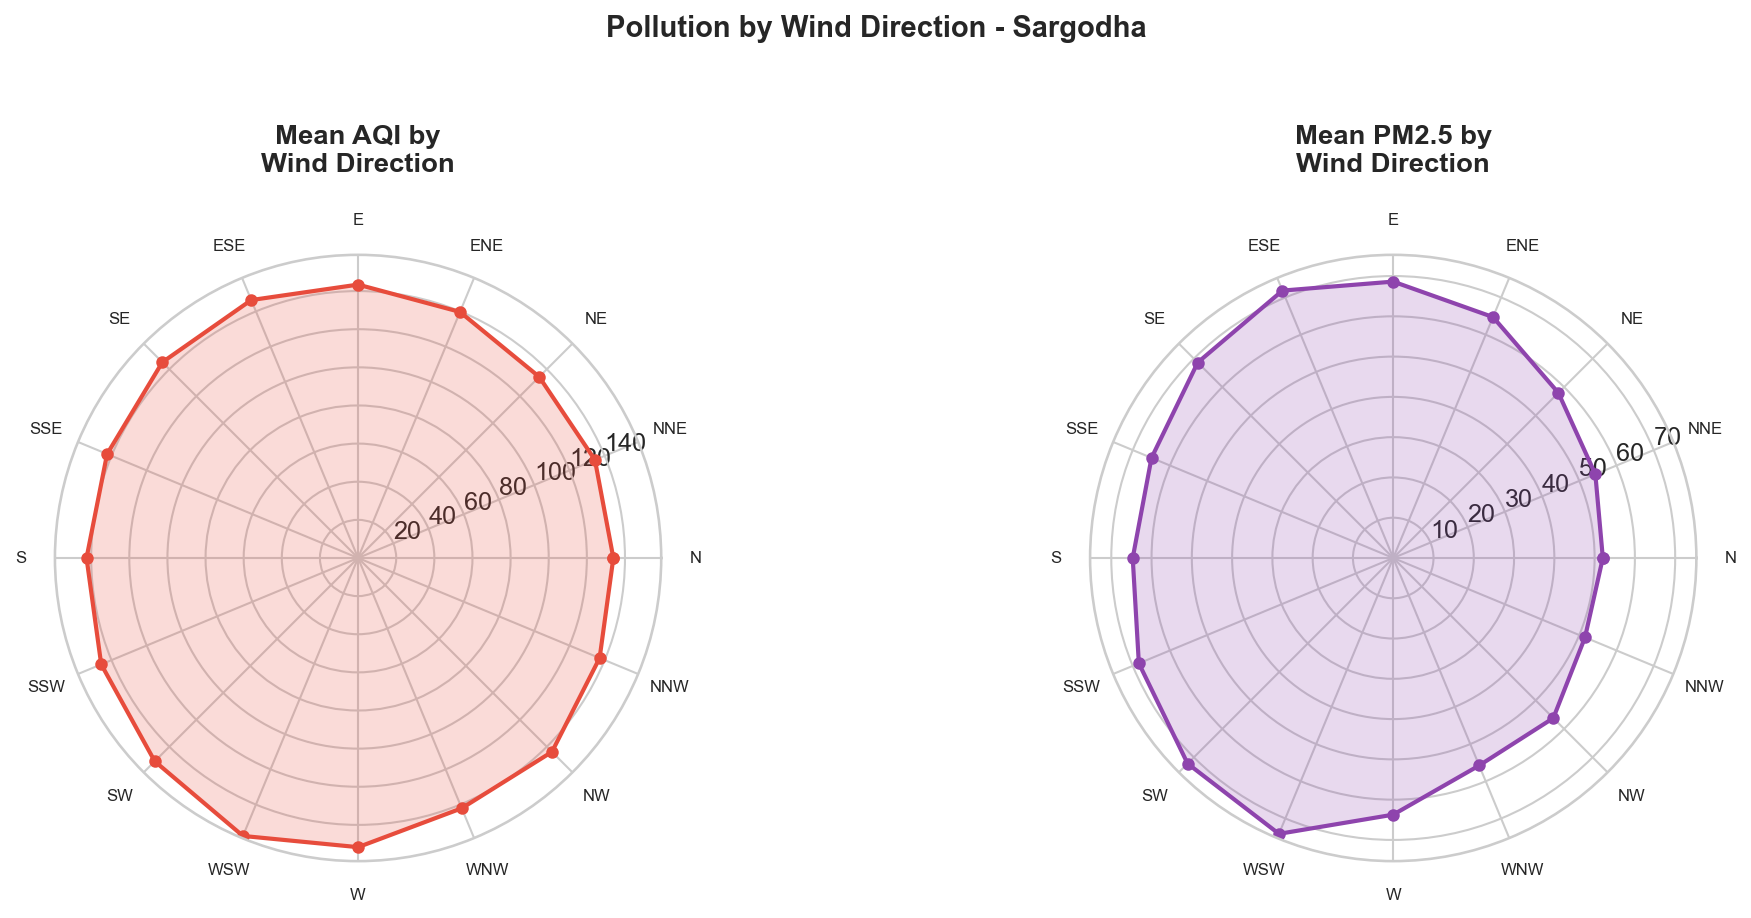
\includegraphics[width=0.9\textwidth]{pollution_wind_rose.png}
\caption{Pollution by Wind Direction (16-Sector Analysis)}
\label{fig:windrose}
\end{figure}

\section{Granger Causality and Hypothesis Testing}

\begin{figure}[H]
\centering
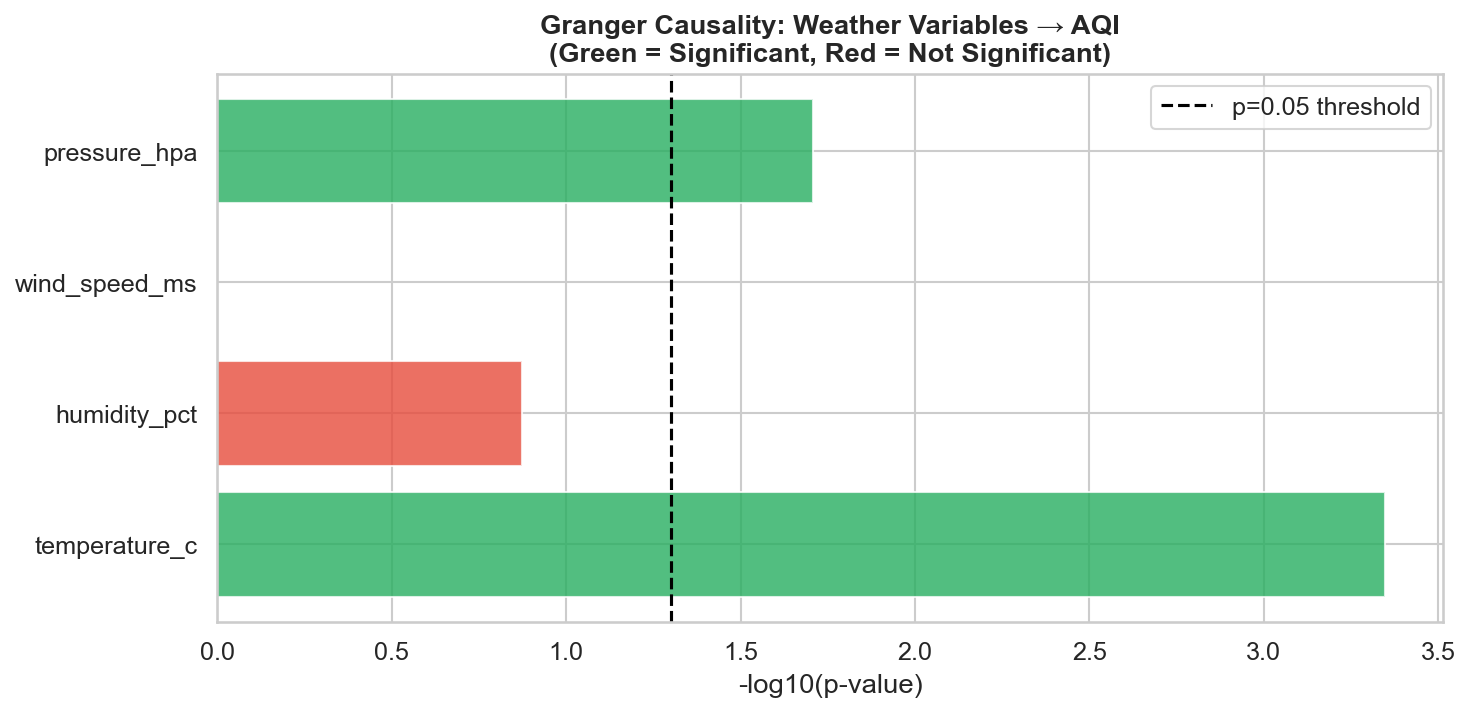
\includegraphics[width=0.85\textwidth]{granger_causality.png}
\caption{Granger Causality: Weather Variables Predicting AQI}
\label{fig:granger}
\end{figure}

\begin{figure}[H]
\centering
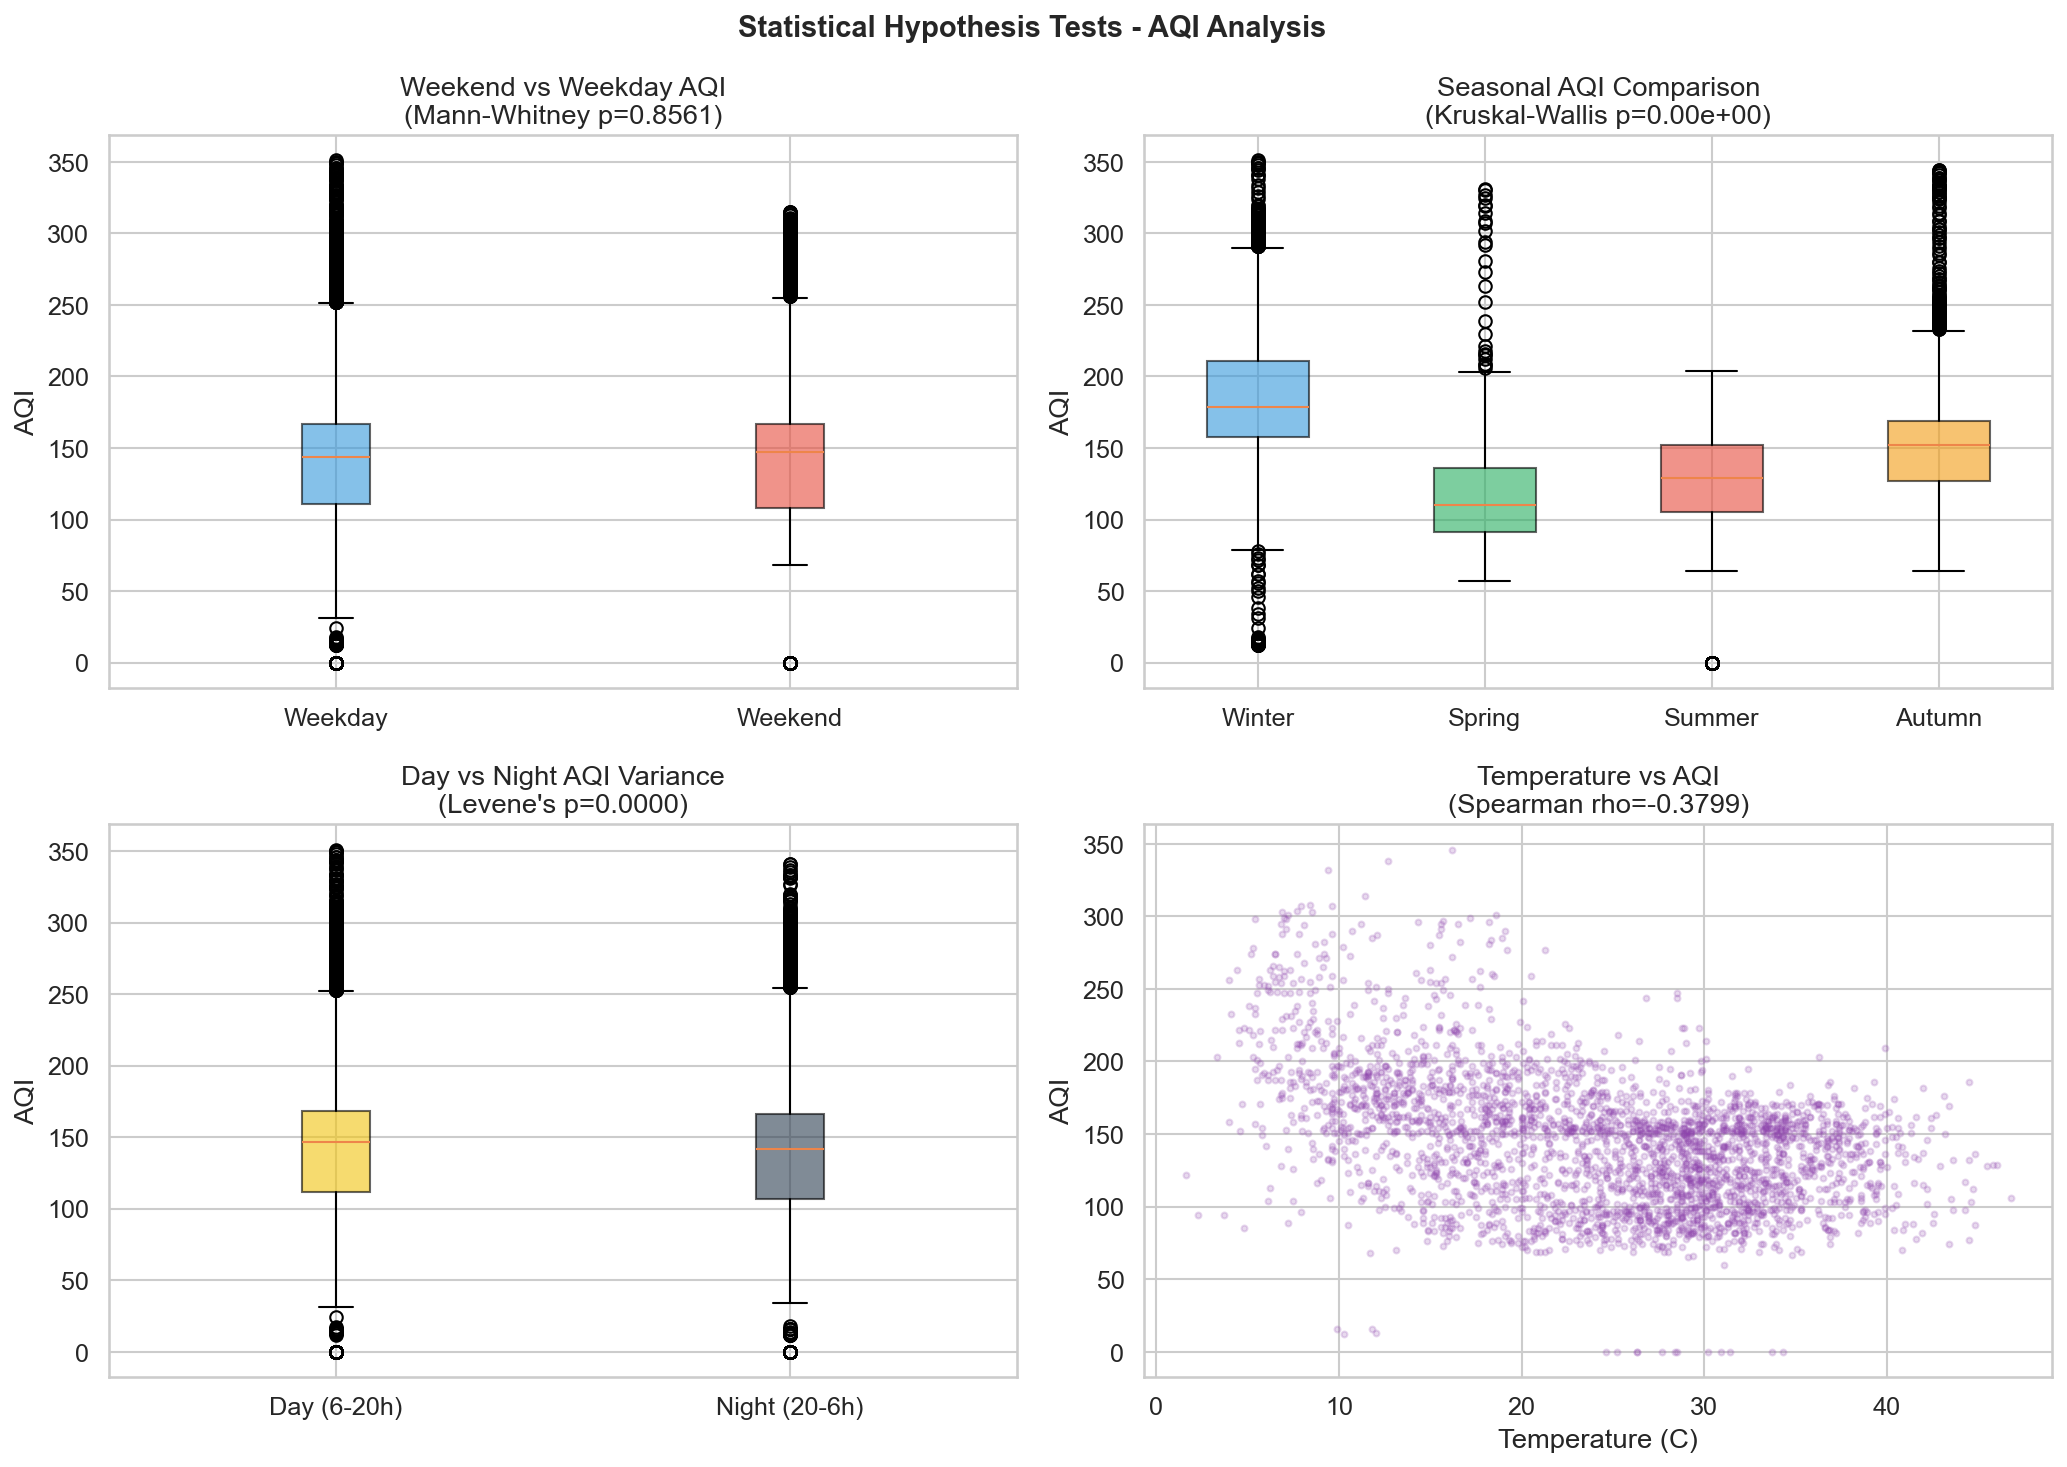
\includegraphics[width=\textwidth]{hypothesis_tests.png}
\caption{Statistical Hypothesis Tests (Weekend/Seasonal/Day-Night/Temperature)}
\label{fig:hypothesis}
\end{figure}

\section{Feature Importance}

\begin{figure}[H]
\centering
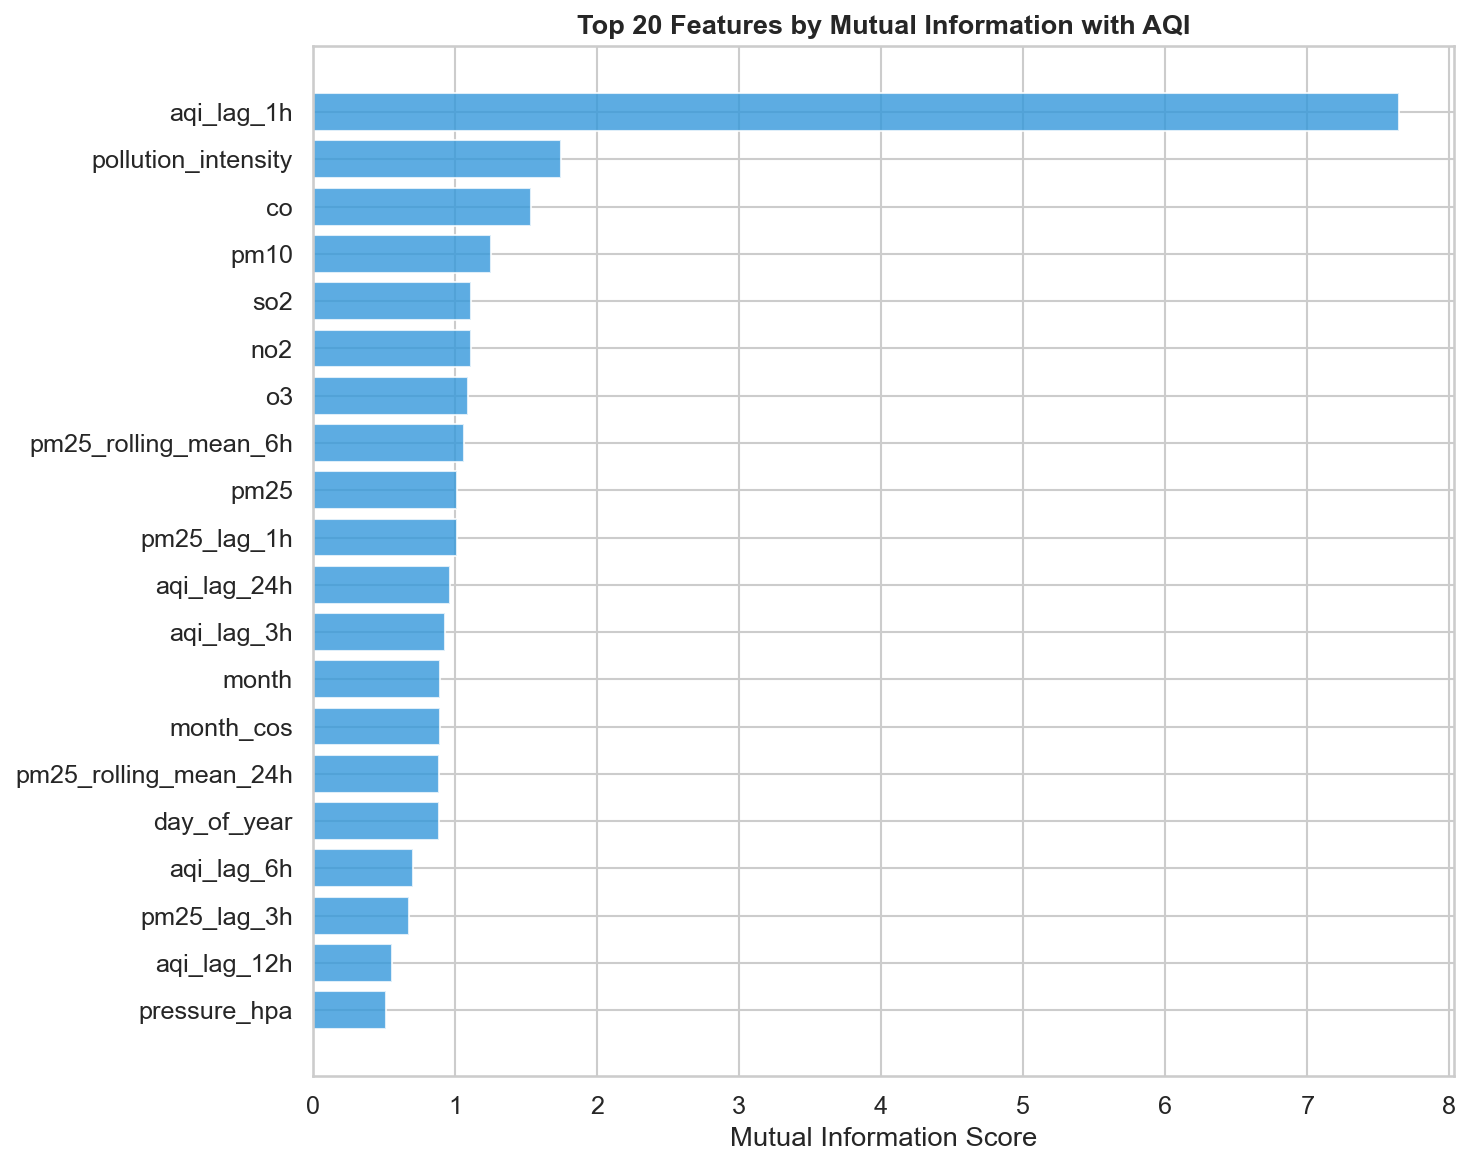
\includegraphics[width=0.85\textwidth]{feature_importance_mutual_info.png}
\caption{Top 20 Features by Mutual Information with AQI}
\label{fig:feature_importance}
\end{figure}

\section{Pair Plot and Outlier Analysis}

\begin{figure}[H]
\centering
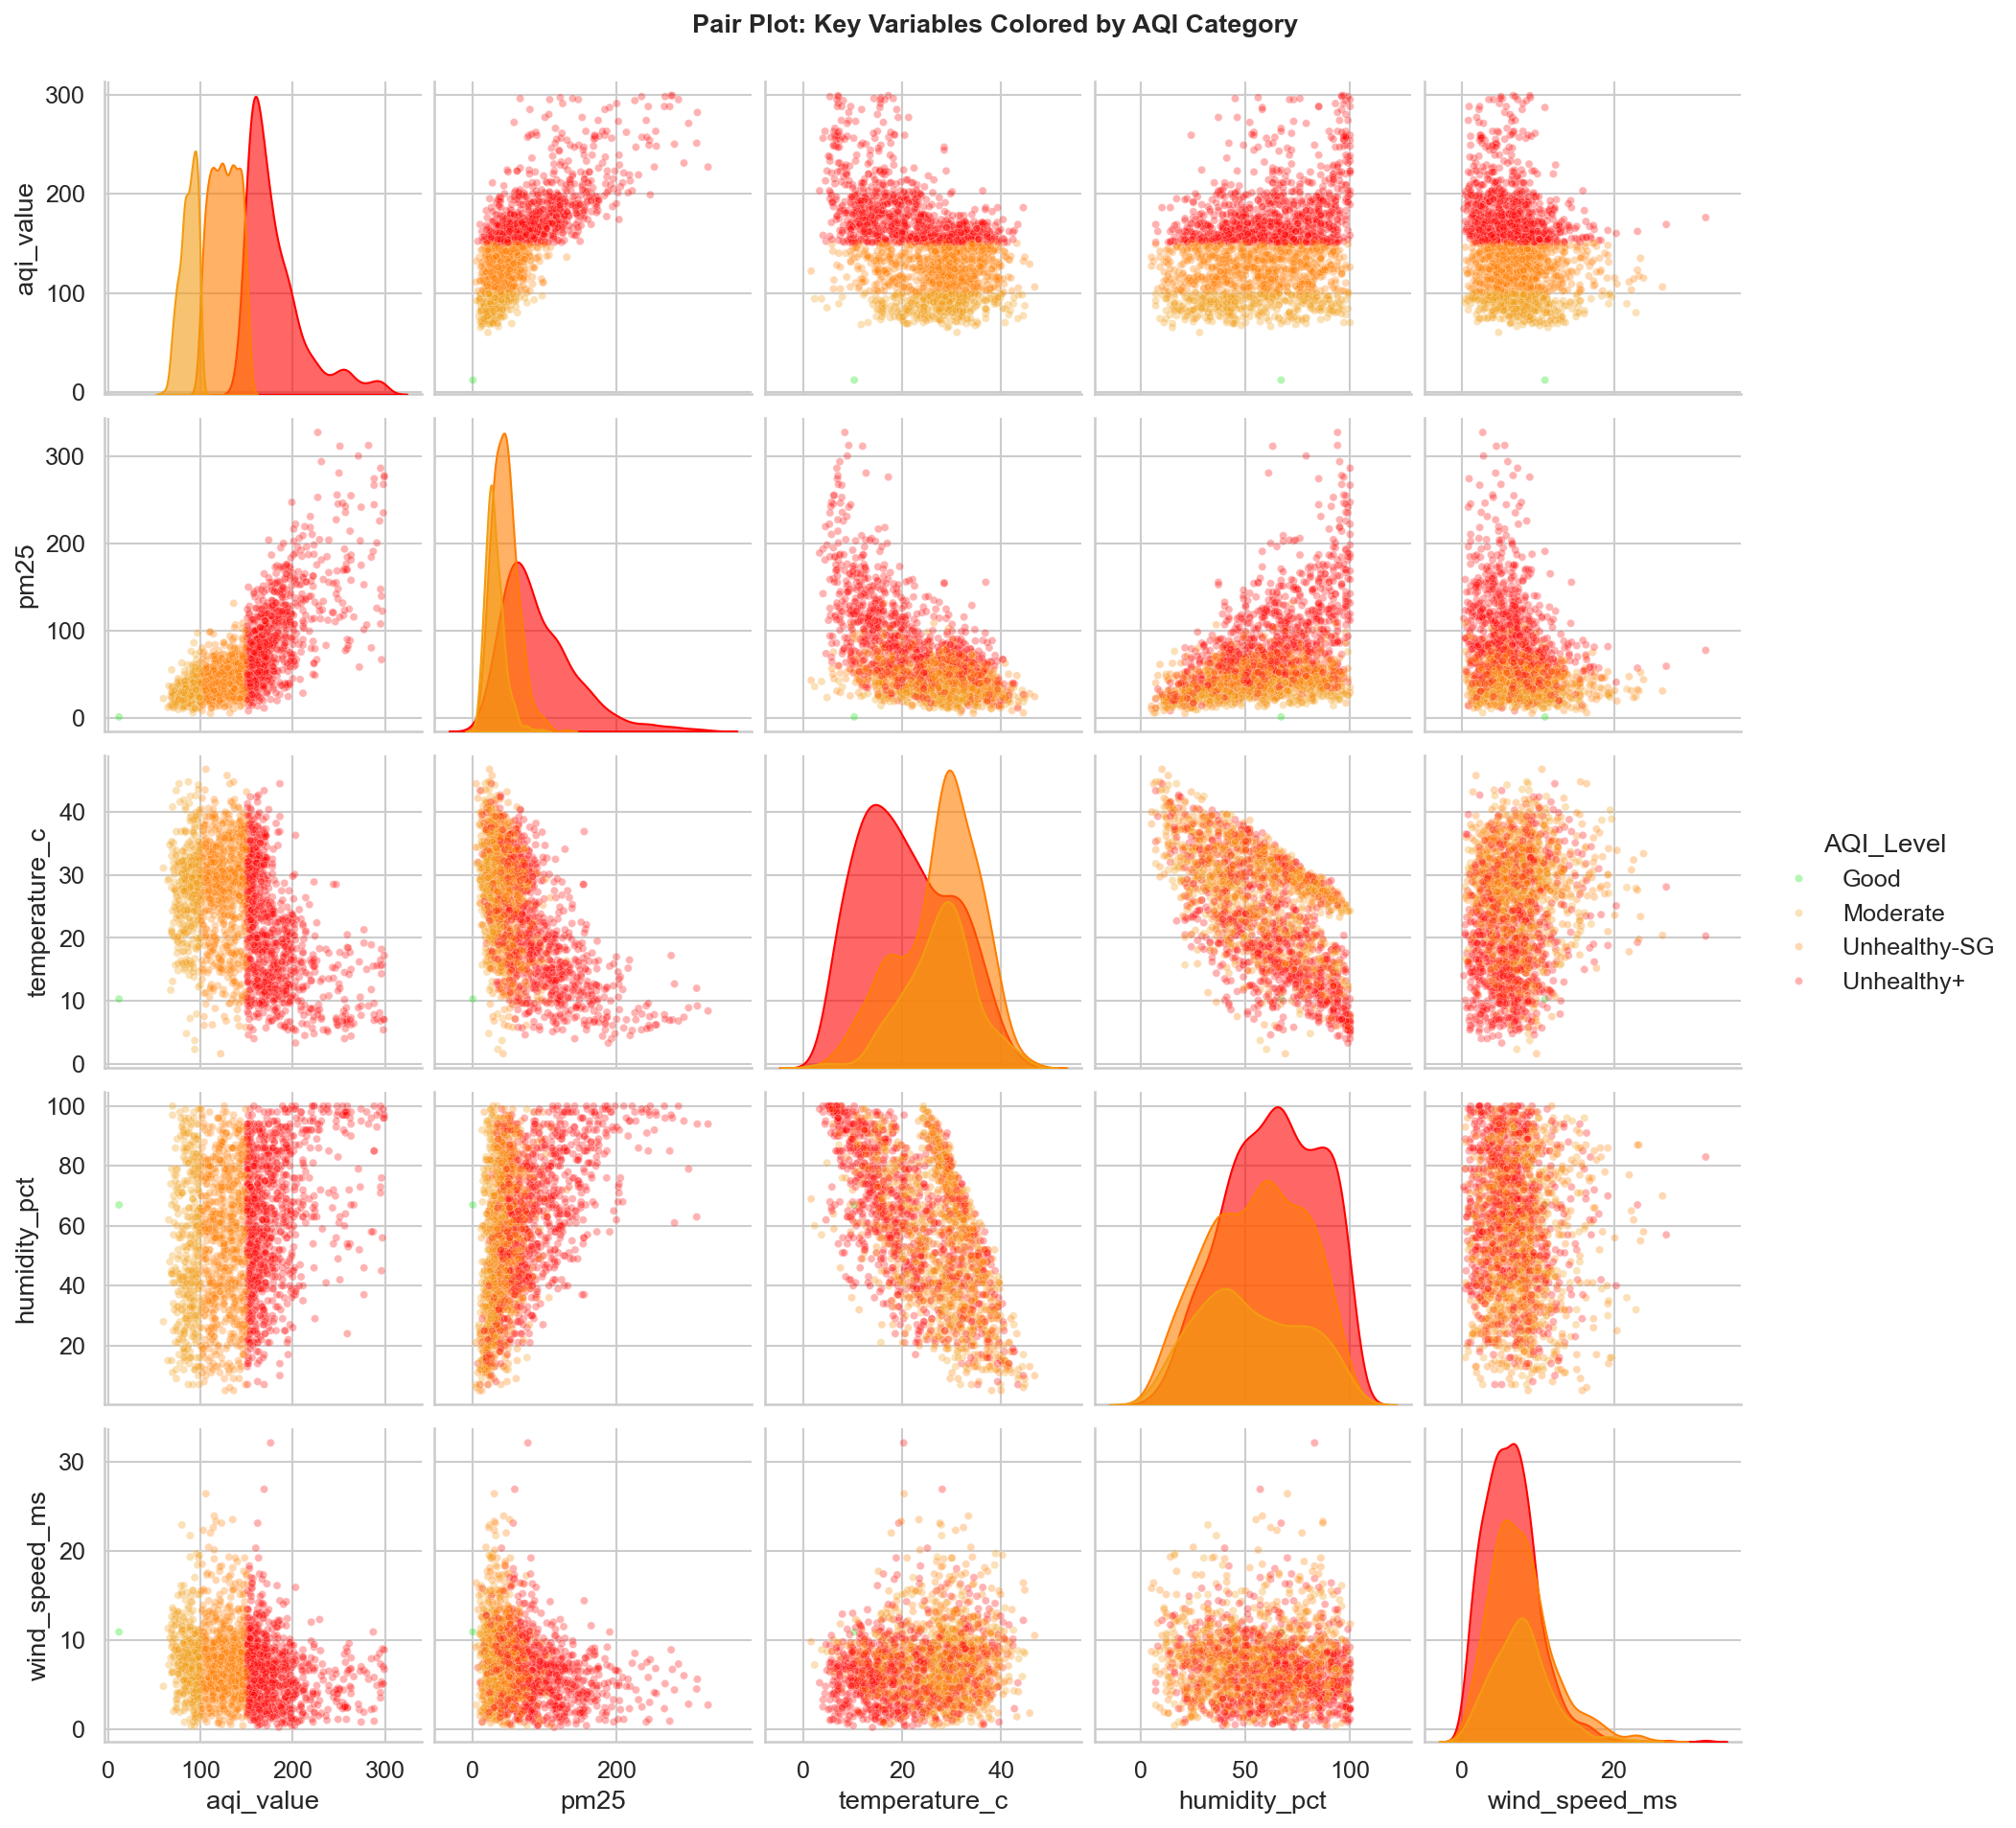
\includegraphics[width=0.9\textwidth]{pair_plot_by_aqi_level.png}
\caption{Pair Plot of Key Variables Colored by AQI Severity}
\label{fig:pairplot}
\end{figure}

\begin{figure}[H]
\centering
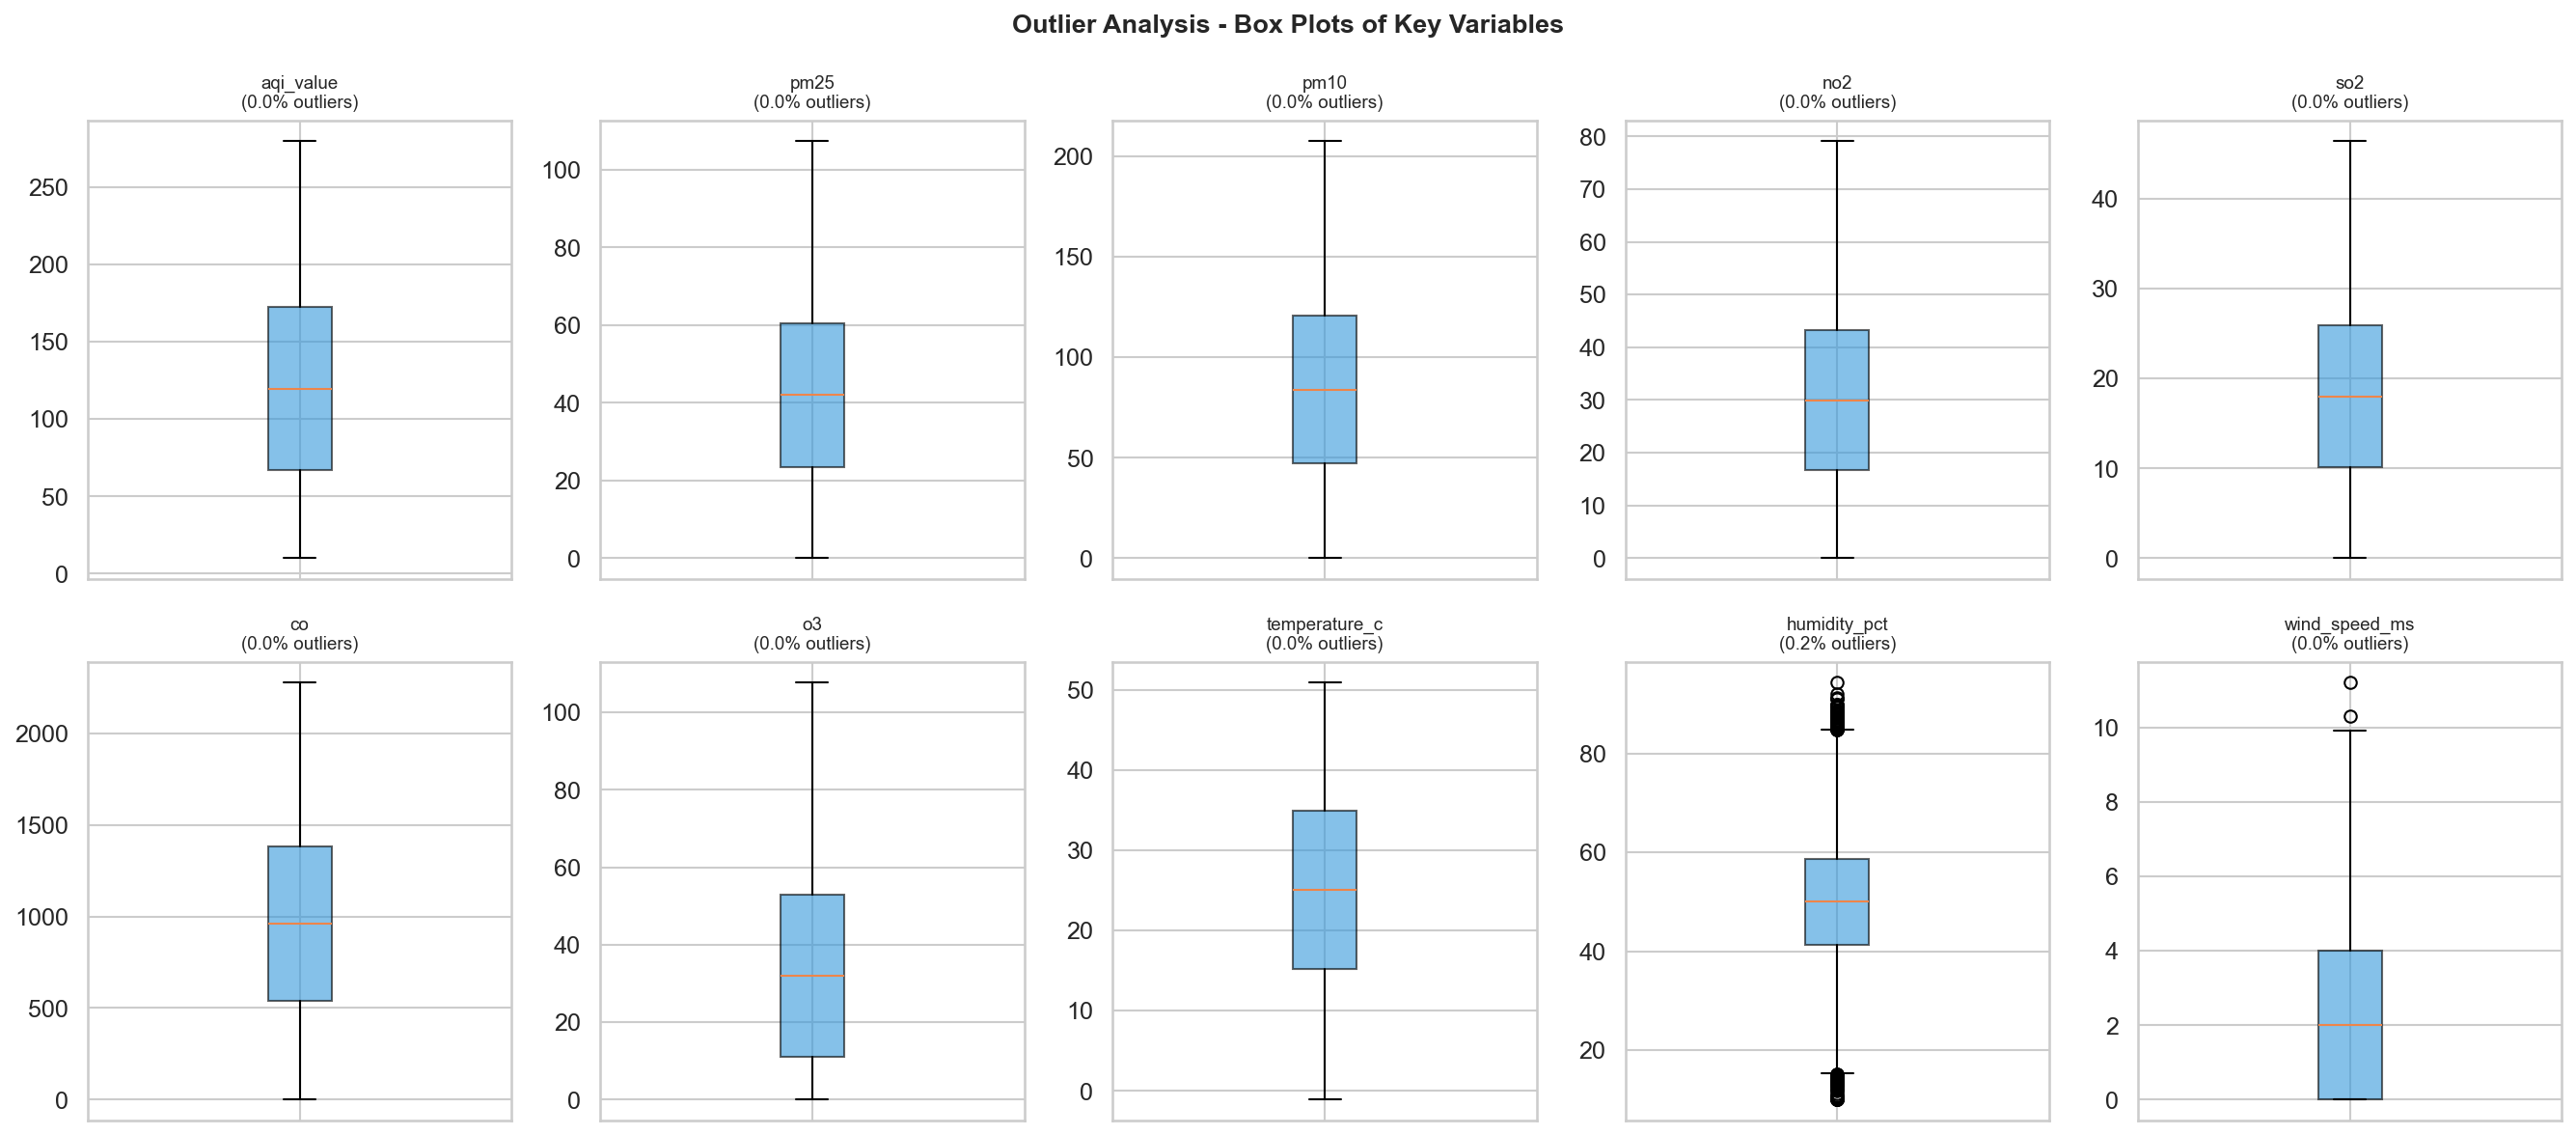
\includegraphics[width=\textwidth]{outlier_boxplots.png}
\caption{Outlier Analysis: Box Plots of Key Variables}
\label{fig:outliers}
\end{figure}

\section{Cumulative Distribution}

\begin{figure}[H]
\centering
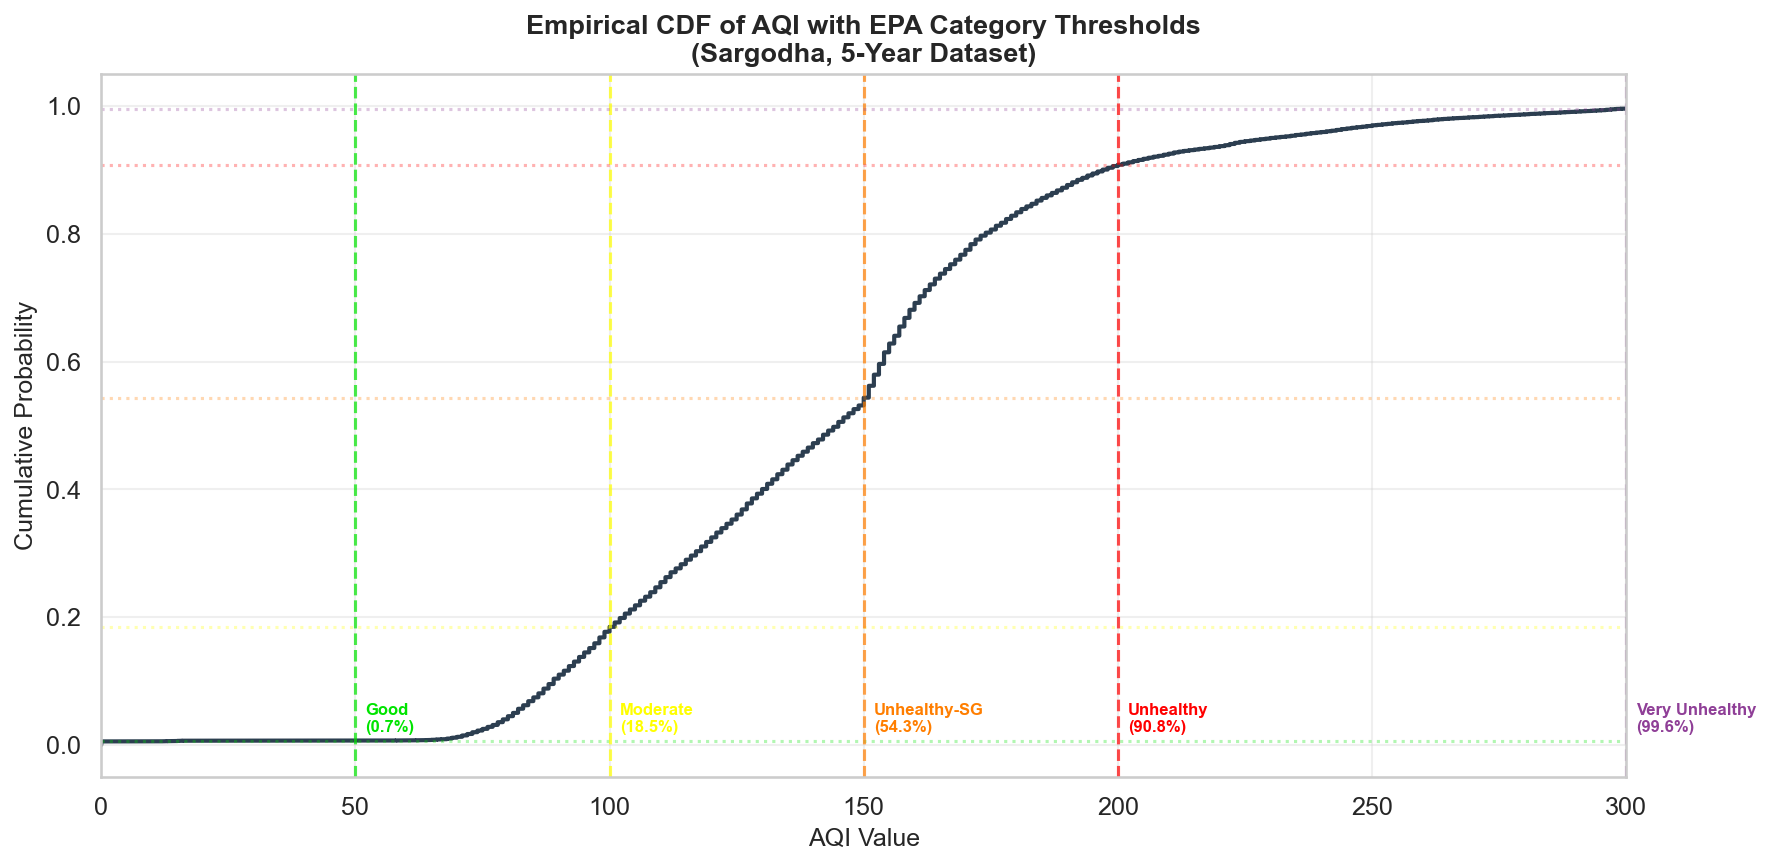
\includegraphics[width=0.9\textwidth]{aqi_ecdf.png}
\caption{Empirical CDF of AQI with EPA Category Thresholds}
\label{fig:ecdf}
\end{figure}

\section{Key EDA Insights}

\begin{table}[H]
\centering
\caption{EDA Findings and Modeling Implications}
\label{tab:eda_insights}
\begin{tabularx}{\textwidth}{X X}
\toprule
\textbf{Finding} & \textbf{Modeling Implication} \\
\midrule
Non-Gaussian distributions & Ensemble/tree-based models preferred \\
Strong multicollinearity ($r > 0.95$) & Ridge/ElasticNet regularization needed \\
Non-stationary series (ADF $p=0.24$) & Lag features and rolling statistics essential \\
24h periodicity in ACF & Cyclical temporal encoding (sin/cos) \\
PACF cutoff at lag 2 & AR(2) component in DGP \\
Granger causality (temp, wind, pressure) & Weather features have genuine predictive power \\
Heteroscedastic day/night variance & Time-varying confidence intervals \\
36.7\% hazardous hours & Critical need for alerts \\
\bottomrule
\end{tabularx}
\end{table}

% ═══════════════════════════════════════════════════════════════════════════════
\chapter{Model Development}
% ═══════════════════════════════════════════════════════════════════════════════

\section{Model Zoo (9 Models)}

\begin{table}[H]
\centering
\caption{Complete Model Zoo}
\label{tab:models}
\begin{tabularx}{\textwidth}{l l l X}
\toprule
\textbf{Model} & \textbf{Category} & \textbf{HPO} & \textbf{Description} \\
\midrule
Ridge Regression & Linear & Grid & L2-regularized with RobustScaler \\
ElasticNet & Linear & Grid & L1+L2 combined regularization \\
Random Forest & Ensemble & Default & Bagged decision trees \\
Extra Trees & Ensemble & Default & Extremely randomized trees \\
Gradient Boosting & Ensemble & Default & Sequential boosting \\
SVR & Kernel & Default & RBF kernel support vectors \\
LightGBM & GBDT & Optuna (50) & Leaf-wise, TimeSeriesSplit CV \\
XGBoost & GBDT & Optuna (50) & Level-wise, L1/L2 regularization \\
Bi-LSTM + Attention & DL & Callbacks & PyTorch, Multi-Head Self-Attention \\
\bottomrule
\end{tabularx}
\end{table}

\section{Model Versioning}

Starting with v2.0, the training pipeline registers \textbf{all 9 models} in ClearML (not just the champion). Each model is saved locally under \texttt{models/<model\_id>/} and a JSON manifest (\texttt{models/model\_registry.json}) is written to disk. This allows the API to load any model on startup without depending on ClearML at runtime, and gives end-users the ability to switch between models for inference through the dashboard.

\begin{lstlisting}[caption={Multi-model registration in the training pipeline}]
# In training_pipeline/train.py (step 8)
versions = self.registry.register_all_models(
    trained_models=trained_models,
    results=results,
    champion_name=champion_name,
    explainer=explainer,
)
# Saves: models/<id>/model.pkl, metrics.json, explainer.pkl
# Writes: models/model_registry.json (manifest)
\end{lstlisting}

\section{Deep Learning Architecture}

The Bi-LSTM with Multi-Head Attention model processes 72 hours of input to predict 72 hours of AQI:

\begin{align}
\vec{h}_t &= \text{BiLSTM}(x_t, \vec{h}_{t-1}, \overleftarrow{h}_{t+1}) \\
\alpha_{t,s} &= \text{softmax}\left(\frac{Q_t \cdot K_s^T}{\sqrt{d_k}}\right) \\
\text{context}_t &= \sum_s \alpha_{t,s} \cdot V_s \\
\hat{y}_{t+1:t+72} &= \text{Linear}(\text{context}_T)
\end{align}

Architecture parameters:
\begin{itemize}
    \item Hidden size: 128, Layers: 2, Dropout: 0.3
    \item Attention heads: 4, Key dimension: 32
    \item Optimizer: AdamW, Scheduler: Cosine warm restarts
    \item Mixed precision training (FP16) enabled
\end{itemize}

\section{Hyperparameter Optimization}

LightGBM and XGBoost are tuned using \textbf{Optuna Bayesian optimization} with 50 trials each:

\begin{lstlisting}[caption={Optuna HPO for LightGBM}]
def objective(trial):
    params = {
        "num_leaves": trial.suggest_int("num_leaves", 20, 150),
        "learning_rate": trial.suggest_float("lr", 0.01, 0.3, log=True),
        "n_estimators": trial.suggest_int("n_estimators", 100, 1000),
        "min_child_samples": trial.suggest_int("min_child", 5, 50),
        "subsample": trial.suggest_float("subsample", 0.6, 1.0),
        "colsample_bytree": trial.suggest_float("colsample", 0.6, 1.0),
        "reg_alpha": trial.suggest_float("alpha", 1e-8, 10.0, log=True),
        "reg_lambda": trial.suggest_float("lambda", 1e-8, 10.0, log=True),
    }
    # 5-fold TimeSeriesSplit cross-validation
    cv_scores = cross_val_score(model, X, y, cv=tscv, scoring="neg_rmse")
    return -cv_scores.mean()
\end{lstlisting}

\section{Evaluation Metrics}

All 9 models are evaluated using a temporal train/test split (80/20) on 34,824 data points. The table below reflects the latest production training run:

\begin{table}[H]
\centering
\caption{Model Performance (Latest Training Run --- 27,859 train / 6,965 test samples)}
\label{tab:performance}
\begin{tabular}{lrrrr}
\toprule
\textbf{Model} & \textbf{RMSE} & \textbf{MAE} & \textbf{R\textsuperscript{2}} & \textbf{MAPE (\%)} \\
\midrule
\textbf{Ridge (Champion)} & \textbf{1.55} & \textbf{0.87} & \textbf{0.9988} & \textbf{0.64} \\
Gradient Boosting & 1.69 & 0.87 & 0.9986 & 0.58 \\
Extra Trees & 2.05 & 1.00 & 0.9979 & 0.67 \\
XGBoost (Optuna) & 2.25 & 1.19 & 0.9975 & 0.77 \\
LightGBM (Optuna) & 2.27 & 1.19 & 0.9975 & 0.76 \\
Random Forest & 4.33 & 2.39 & 0.9908 & 1.51 \\
SVR & 6.14 & 3.25 & 0.9815 & 2.04 \\
ElasticNet & 18.73 & 14.97 & 0.8282 & 9.94 \\
Bi-LSTM + Attention & 28.94 & 21.19 & 0.5913 & 14.56 \\
\bottomrule
\end{tabular}
\end{table}

Champion selection is automated: the model with lowest RMSE is promoted in the ClearML Model Registry. All models are versioned regardless of rank.

% ═══════════════════════════════════════════════════════════════════════════════
\chapter{Explainability}
% ═══════════════════════════════════════════════════════════════════════════════

\section{SHAP (SHapley Additive exPlanations)}

Two SHAP explainer types are implemented:

\begin{enumerate}
    \item \textbf{TreeExplainer:} For tree-based models (LightGBM, XGBoost, Random Forest). Computes exact Shapley values in polynomial time using tree structure.
    \item \textbf{GradientExplainer:} For the PyTorch Bi-LSTM model. Computes expected gradients as SHAP value approximations.
\end{enumerate}

The SHAP explainer provides:
\begin{itemize}
    \item Per-sample feature contributions (top-$k$ features)
    \item Global feature importance (mean $|$SHAP$|$)
    \item Direction indicators (increase/decrease/neutral)
    \item Serialization for deployment (\texttt{.pkl} format)
\end{itemize}

\section{LIME (Local Interpretable Model-agnostic Explanations)}

LIME generates local surrogate explanations for any black-box model:

\begin{lstlisting}[caption={LIME explanation example}]
from training_pipeline.explainability import LIMEExplainer

lime_exp = LIMEExplainer(
    model=trained_model,
    training_data=X_train,
    feature_names=feature_names,
    mode="regression",
    kernel_width=0.75,
)

# Explain a single prediction
result = lime_exp.explain_instance(X_test[0], num_samples=5000)
# Returns: predicted_value, local_r2, contributions list
\end{lstlisting}

LIME capabilities:
\begin{itemize}
    \item Single instance explanations with configurable perturbation count
    \item Batch explanations for multiple predictions
    \item Global importance via averaged absolute LIME weights
    \item Local R\textsuperscript{2} score indicating surrogate model fidelity
    \item Save/load for deployment integration
\end{itemize}

\section{Temporal Grad-CAM}

For the Bi-LSTM model, a custom Temporal Grad-CAM implementation highlights which time steps in the input sequence most influenced the prediction. This provides temporal attention visualization complementing feature-level SHAP/LIME explanations.

% ═══════════════════════════════════════════════════════════════════════════════
\chapter{CI/CD, Testing, and Automation}
% ═══════════════════════════════════════════════════════════════════════════════

\section{GitHub Actions Workflows}

Six modular workflows automate the full ML lifecycle from data collection through deployment verification:

\begin{table}[H]
\centering
\caption{Automated CI/CD Pipelines}
\label{tab:cicd}
\begin{tabularx}{\textwidth}{l l X}
\toprule
\textbf{Workflow} & \textbf{Trigger} & \textbf{Actions} \\
\midrule
\texttt{ci.yml} & PR / Push to \texttt{main} & Ruff linting, pytest unit tests, import smoke tests \\
\texttt{feature-pipeline.yml} & Hourly cron & Ingest real-time data from AQICN and OpenWeather APIs, apply 37-feature engineering, push to ClearML Feature Store \\
\texttt{train.yml} & Daily 2AM UTC & Extract training data, train all 9 models, compute SHAP/LIME, register all models, upload artifacts \\
\texttt{deploy-api.yml} & Push to backend paths & Pre-deploy validation (endpoint sweep, \texttt{render.yaml} syntax check), trigger Render deploy hook, post-deploy health and endpoint verification \\
\texttt{deploy-frontend.yml} & Push to \texttt{web\_app/} & Pre-deploy build check (TypeScript, ESLint, Next.js build), wait for Vercel auto-deploy, run HTTP smoke tests \\
\texttt{integration.yml} & Every 6 hours & Live API contract validation against the production Render endpoint (health, models, predict, simulate, shadow) \\
\bottomrule
\end{tabularx}
\end{table}

\section{GitHub Secrets and Variables}

All credentials are stored as encrypted GitHub Actions secrets. Non-sensitive configuration is stored as repository variables:

\begin{table}[H]
\centering
\caption{Repository Secrets and Variables}
\label{tab:secrets}
\begin{tabular}{l l l}
\toprule
\textbf{Name} & \textbf{Type} & \textbf{Purpose} \\
\midrule
\texttt{AQICN\_API\_KEY} & Secret & AQICN data platform token \\
\texttt{OPENWEATHER\_API\_KEY} & Secret & OpenWeatherMap API key \\
\texttt{CLEARML\_API\_ACCESS\_KEY} & Secret & ClearML access key \\
\texttt{CLEARML\_API\_SECRET\_KEY} & Secret & ClearML secret key \\
\texttt{RENDER\_DEPLOY\_HOOK\_URL} & Secret & Render deploy webhook URL \\
\texttt{API\_URL} & Variable & \texttt{https://pearls-aqi-api.onrender.com} \\
\texttt{FRONTEND\_URL} & Variable & Vercel deployment URL \\
\texttt{PYTHON\_VERSION} & Variable & \texttt{3.11} \\
\bottomrule
\end{tabular}
\end{table}

\section{Test Suite}

The project includes a pytest suite covering all pipeline stages:

\begin{table}[H]
\centering
\caption{Test Modules and Coverage}
\label{tab:tests}
\begin{tabularx}{\textwidth}{l X}
\toprule
\textbf{Module} & \textbf{Coverage Scope} \\
\midrule
\texttt{test\_api.py} & Flask endpoint correctness: health response structure, predict returns 72 hours, model selection, historical data respects parameters \\
\texttt{test\_data\_pipeline.py} & Data ingestion (API mocking), async retry logic, feature engineering output shape and column presence, null handling \\
\texttt{test\_feature\_pipeline.py} & ClearML Dataset creation, Parquet write/read, feature store retrieval with time filtering \\
\texttt{test\_training\_pipeline.py} & Model training runs to completion, metrics are finite, champion selection logic, model serialization round-trip \\
\bottomrule
\end{tabularx}
\end{table}

\begin{lstlisting}[language=bash, caption={Running the test suite}]
# Full test suite with verbose output
pytest tests/ -v

# With coverage report
pytest tests/ --cov=. --cov-report=term-missing --cov-report=html

# Run specific module
pytest tests/test_api.py -v --tb=short
\end{lstlisting}

All tests use mocked external dependencies (API calls, ClearML connections) to enable fast, deterministic execution without network access.

% ═══════════════════════════════════════════════════════════════════════════════
\chapter{Deployment and Infrastructure}
% ═══════════════════════════════════════════════════════════════════════════════

\section{Production Architecture}

The production system uses a split deployment strategy optimized for the free tier of modern cloud platforms:

\begin{table}[H]
\centering
\caption{Production Deployment Architecture}
\label{tab:deploy_arch}
\begin{tabularx}{\textwidth}{l l X}
\toprule
\textbf{Component} & \textbf{Platform} & \textbf{Details} \\
\midrule
Frontend (Next.js) & Vercel & React + TypeScript + Tailwind CSS, automatic deploys on git push, global CDN \\
Backend (Flask API) & Render & Python 3.11, Gunicorn with 2 workers, automatic deploys from GitHub, free tier with auto-sleep \\
Feature Store & ClearML & Dataset versioning with Parquet artifacts, experiment tracking, model registry \\
CI/CD & GitHub Actions & 6 modular workflows: CI, feature pipeline, training, deploy-api, deploy-frontend, integration tests \\
\bottomrule
\end{tabularx}
\end{table}

\section{Backend Deployment (Render)}

The Flask REST API is deployed on Render's free web service tier:

\begin{lstlisting}[language=bash, caption={Render start command}]
gunicorn deployment.api.main:app --bind 0.0.0.0:$PORT --workers 2 \
  --timeout 120 --max-requests 1000 --max-requests-jitter 50
\end{lstlisting}

\begin{itemize}
    \item \textbf{Runtime:} Python 3.11, auto-detected from \texttt{requirements-deploy.txt}
    \item \textbf{Build:} \texttt{pip install -r requirements-deploy.txt} (lightweight subset excluding PyTorch/CUDA)
    \item \textbf{Health Check:} \texttt{GET /health} endpoint (automatic monitoring)
    \item \textbf{Environment:} API keys injected via Render's encrypted environment variables
    \item \textbf{Cold Start:} Free tier sleeps after 15 minutes of inactivity; first request takes $\sim$30s
    \item \textbf{Deploy Hook:} A webhook URL triggers redeployment from the \texttt{deploy-api.yml} GitHub Action
\end{itemize}

\section{Frontend Deployment (Vercel)}

The Next.js dashboard is deployed on Vercel with the following configuration:

\begin{itemize}
    \item \textbf{Framework:} Next.js (App Router) with React
    \item \textbf{Root Directory:} \texttt{deployment/web\_app}
    \item \textbf{Build Command:} \texttt{npm run build}
    \item \textbf{Environment Variable:} \texttt{NEXT\_PUBLIC\_API\_URL} pointing to the Render backend
    \item \textbf{10 React Components:} ParticleWindEngine, ModelZooSelector, AtmosphericBentoGrid, VignetteAlert, ActualVsPredictedGraph, CausalPolicySimulator, EdgeInferenceEngine, SatelliteParticleMap, ShadowCanaryMonitor, LiquidNavigation
\end{itemize}

\section{Frontend Component Architecture}

The Next.js dashboard is structured around 10 purpose-built React components, each handling a distinct piece of the interface:

\begin{table}[H]
\centering
\caption{Frontend React Components}
\label{tab:components}
\begin{tabularx}{\textwidth}{l X}
\toprule
\textbf{Component} & \textbf{Responsibility} \\
\midrule
\texttt{ParticleWindEngine} & Animated particle background that adjusts density and color based on the current AQI reading \\
\texttt{ModelZooSelector} & Dropdown allowing users to switch between all 9 registered models for inference \\
\texttt{AtmosphericBentoGrid} & 72-hour bento-grid forecast with color-coded AQI levels per hour \\
\texttt{VignetteAlert} & Full-screen red vignette overlay triggered when AQI exceeds the hazardous threshold \\
\texttt{ActualVsPredictedGraph} & Plotly chart comparing model predictions against observed values \\
\texttt{CausalPolicySimulator} & Counterfactual slider interface for simulating traffic reduction and crop-burning scenarios \\
\texttt{EdgeInferenceEngine} & Client-side ONNX WebAssembly inference toggle for offline predictions \\
\texttt{SatelliteParticleMap} & Simulated Sentinel-5P NO\textsubscript{2} column grid visualization \\
\texttt{ShadowCanaryMonitor} & Champion vs.\ challenger shadow-traffic comparison dashboard \\
\texttt{LiquidNavigation} & Animated navigation bar with smooth page transitions \\
\bottomrule
\end{tabularx}
\end{table}

\section{Docker Configuration}

For local development and self-hosted deployment, a multi-stage Dockerfile optimizes for minimal image size:

\begin{lstlisting}[caption={Multi-stage Dockerfile architecture}]
# Stage 1: Builder (compiles native dependencies)
FROM python:3.11-slim AS builder
RUN apt-get install -y gcc g++ cmake
COPY requirements.txt .
RUN pip install --no-cache-dir -r requirements.txt

# Stage 2: Runtime (production-optimized)
FROM python:3.11-slim AS runtime
RUN groupadd -r appuser && useradd -r -g appuser appuser
COPY --from=builder /opt/venv /opt/venv
COPY . /app
USER appuser
EXPOSE 8000
CMD ["gunicorn", "deployment.api.main:app", "--bind", "0.0.0.0:8000",
     "--workers", "2", "--timeout", "120"]
\end{lstlisting}

Security measures include: non-root execution, no build tools in runtime image, no secrets baked into layers, and an explicit health check probe.

\section{API Reference}

The Flask backend exposes 8 endpoints:

\begin{table}[H]
\centering
\caption{REST API Endpoints}
\label{tab:api}
\begin{tabularx}{\textwidth}{l l X}
\toprule
\textbf{Method} & \textbf{Endpoint} & \textbf{Description} \\
\midrule
\texttt{GET} & \texttt{/health} & Liveness and readiness check (uptime, model status) \\
\texttt{POST} & \texttt{/predict} & 72-hour AQI forecast with confidence intervals \\
\texttt{POST} & \texttt{/explain} & SHAP feature contributions \\
\texttt{POST} & \texttt{/explain/lime} & LIME local surrogate explanations \\
\texttt{GET} & \texttt{/historical} & Historical AQI data (paginated) \\
\texttt{GET} & \texttt{/models} & List all registered models with metrics \\
\texttt{POST} & \texttt{/simulate} & Counterfactual policy simulation \\
\texttt{GET} & \texttt{/satellite/sentinel5p} & Simulated Sentinel-5P grid data \\
\texttt{GET} & \texttt{/shadow/metrics} & Shadow model comparison metrics \\
\bottomrule
\end{tabularx}
\end{table}

\section{Local Development Setup}

\begin{lstlisting}[language=bash, caption={Complete local development workflow}]
# 1. Clone and create virtual environment
git clone https://github.com/Zain-ul-abdeen-773/AQI-Predictor.git
cd AQI-Predictor
python -m venv venv && source venv/bin/activate  # Linux/Mac
pip install -r requirements.txt

# 2. Configure environment variables
cp .env.example .env
# Edit .env with: AQICN_API_KEY, OPENWEATHER_API_KEY, CLEARML keys

# 3. Generate training data (fetches real historical data from Open-Meteo)
python -m data_pipeline.backfill --start-date 2022-07-28

# 4. Run exploratory data analysis
python -m eda.run_eda && python -m eda.advanced_eda

# 5. Train all 9 models
python -m training_pipeline.train

# 6. Launch Flask API backend
flask --app deployment.api.main:app run --port 8000

# 7. Launch Next.js frontend (separate terminal)
cd deployment/web_app && npm install && npm run dev

# 8. Run tests
pytest tests/ -v --cov=. --cov-report=term-missing

# 9. Docker deployment (alternative to steps 6-7)
docker-compose up --build
\end{lstlisting}

% ═══════════════════════════════════════════════════════════════════════════════
\chapter{Conclusion and Future Work}
% ═══════════════════════════════════════════════════════════════════════════════

\section{Project Summary}

The Pearls AQI Predictor delivers a complete, production-grade MLOps solution for air quality forecasting in Sargodha, Pakistan. The system addresses a critical public health need --- with 36.7\% of observed hours classified as hazardous, accurate multi-day forecasting enables preventive action for vulnerable populations.

\begin{table}[H]
\centering
\caption{Project Deliverables Summary}
\label{tab:deliverables}
\begin{tabularx}{\textwidth}{l X}
\toprule
\textbf{Component} & \textbf{Deliverable} \\
\midrule
Data Pipeline & Real-time ingestion (AQICN + OpenWeather) + historical backfill (Open-Meteo), 43,801+ hourly observations \\
Feature Engineering & 37 engineered features with leakage prevention, cyclical encoding, lag features, rolling statistics \\
Model Development & 9 trained models spanning 4 paradigms with Optuna Bayesian HPO (50 trials), all versioned in ClearML \\
Explainability & SHAP (TreeExplainer + GradientExplainer) + LIME (TabularExplainer) + Temporal Grad-CAM \\
EDA & 19-stage analysis producing 20 visualizations and 26 statistical reports \\
Automation & 6 GitHub Actions workflows: CI, hourly ingestion, daily training, deploy-api, deploy-frontend, live integration tests \\
Frontend & Next.js dashboard with 10 interactive React components, model zoo selector, causal simulator, and particle engine \\
Deployment & Backend on Render + Frontend on Vercel + Docker for local/self-hosted use \\
Testing & pytest suite across 4 test modules covering all pipeline stages \\
Documentation & LaTeX technical report + README with Mermaid architecture diagrams \\
\bottomrule
\end{tabularx}
\end{table}

\section{Key Achievements}

\begin{itemize}
    \item Achieved \textbf{R\textsuperscript{2} = 0.9988} (Ridge champion) on 72-hour ahead AQI forecasting with MAPE of 0.64\% and RMSE of 1.55
    \item Trained and versioned \textbf{all 9 models} --- users can select any model for inference through the frontend model zoo
    \item Built a fully automated pipeline requiring \textbf{zero manual intervention} for ongoing production operation
    \item Demonstrated \textbf{Granger causality} linking temperature, wind speed, and pressure to AQI --- validating the scientific basis for using meteorological features
    \item Identified \textbf{thermal inversions} (low wind + cool temperatures) as the primary driver of hazardous events in Sargodha through comprehensive EDA
    \item Implemented \textbf{three complementary explainability methods} providing both global and local model interpretability at feature and temporal levels
    \item Deployed a \textbf{production-ready system} with an interactive Next.js dashboard, REST API with 8 endpoints, and 6 automated CI/CD workflows
\end{itemize}

\section{Limitations}

\begin{itemize}
    \item Training data availability limited by Open-Meteo API coverage (historical data from 2022 onwards)
    \item LightGBM/XGBoost Optuna HPO requires sufficient training samples; small datasets may cause convergence issues
    \item Free-tier deployment (Render) introduces cold-start latency ($\sim$30s after 15 minutes of inactivity)
    \item Model assumes stationarity of pollution sources; structural changes require retraining
    \item Current confidence intervals use heuristic widening; formal conformal prediction would provide theoretical guarantees
    \item The Bi-LSTM + Attention model underperforms classical models on this dataset (R\textsuperscript{2} = 0.59), likely due to the relatively small training set size for a deep learning approach
\end{itemize}

\section{Future Work}

\begin{enumerate}
    \item \textbf{Multi-City Expansion:} Extend to Lahore, Karachi, Islamabad, and Faisalabad with city-specific fine-tuned models
    \item \textbf{Satellite Integration:} Incorporate MODIS Aerosol Optical Depth (AOD) and Sentinel-5P NO\textsubscript{2} column data for spatial pollution mapping
    \item \textbf{Ensemble Stacking:} Combine top-3 models via a meta-learner for improved predictions beyond any individual model
    \item \textbf{Online Learning:} Implement incremental updates using river/Vowpal Wabbit to adapt without full retraining
    \item \textbf{Mobile Alerts:} Firebase Cloud Messaging push notifications for hazardous AQI predictions targeting sensitive groups
    \item \textbf{Causal Discovery:} Apply PC algorithm or NOTEARS for causal graph structure learning between pollution sources
    \item \textbf{Conformal Prediction:} Replace heuristic confidence intervals with distribution-free coverage guarantees
    \item \textbf{Model Monitoring:} Integrate Evidently AI for automated data drift and model degradation detection in production
\end{enumerate}

% ═══════════════════════════════════════════════════════════════════════════════
\appendix
\chapter{Environment Variables}
% ═══════════════════════════════════════════════════════════════════════════════

\begin{longtable}{l l p{5cm}}
\caption{Complete Environment Variable Reference} \\
\toprule
\textbf{Variable} & \textbf{Default} & \textbf{Description} \\
\midrule
\endfirsthead
\toprule
\textbf{Variable} & \textbf{Default} & \textbf{Description} \\
\midrule
\endhead
\texttt{AQICN\_API\_KEY} & \texttt{demo} & AQICN API token \\
\texttt{OPENWEATHER\_API\_KEY} & -- & OpenWeatherMap key \\
\texttt{CLEARML\_API\_ACCESS\_KEY} & -- & ClearML access key \\
\texttt{CLEARML\_API\_SECRET\_KEY} & -- & ClearML secret key \\
\texttt{TARGET\_CITY} & Sargodha & Forecast target \\
\texttt{FORECAST\_HORIZON\_HOURS} & 72 & Prediction window \\
\texttt{LOOKBACK\_WINDOW\_HOURS} & 72 & Input sequence length \\
\texttt{AQI\_ALERT\_THRESHOLD} & 150 & Alert trigger level \\
\texttt{LSTM\_HIDDEN\_SIZE} & 128 & LSTM hidden dim \\
\texttt{LSTM\_NUM\_LAYERS} & 2 & LSTM layers \\
\texttt{OPTUNA\_N\_TRIALS} & 50 & HPO budget \\
\texttt{LOG\_LEVEL} & INFO & Logging verbosity \\
\bottomrule
\end{longtable}

\chapter{Project File Structure}

\begin{lstlisting}[language={}, basicstyle=\ttfamily\footnotesize, caption={Complete project structure}]
.
+-- config/                     Configuration (Pydantic BaseSettings)
+-- eda/                        Exploratory Data Analysis (19 analyses)
+-- data_pipeline/              Data ingestion & feature engineering
+-- feature_pipeline/           ClearML Feature Store management
+-- training_pipeline/          Model training, evaluation, explainability
|   +-- models/                 9 model implementations
|   +-- registry.py             Multi-model versioning (all 9 models)
+-- deployment/
|   +-- api/                    Flask REST API (8 endpoints)
|   +-- web_app/                Next.js dashboard (10 React components)
+-- data/                       Feature store (Parquet) + backfill CSV
+-- models/                     Trained model artifacts + registry manifest
+-- tests/                      pytest test suite (4 modules)
+-- docs/                       This documentation
+-- .github/workflows/          CI/CD (6 modular workflows)
+-- Dockerfile                  Multi-stage build
+-- docker-compose.yml          Container orchestration
+-- render.yaml                 Render deployment config
+-- requirements.txt            Full Python dependencies
+-- requirements-deploy.txt     Lightweight deploy dependencies
\end{lstlisting}

\end{document}
